% -*- coding: utf-8 -*-
% !TEX program = latexmk -outdir=./build -pdflatex=lualatex -synctex=1 -interaction=nonstopmode -file-line-error -pdf
\documentclass[final,xcolor={cmyk,hyperref}]{beamer}
\usepackage[orientation=portrait, size=a0, scale=1.25]{beamerposter}
\usepackage{pdfrender}
\usepackage[pdf15,x-1a1]{pdfx}
\FOGRAXXXIX
\usepackage[prefix=]{xcolor-material}
\usepackage{baap-2018-poster}
\usepackage{multicol}
%\usepackage[allfiguresdraft]{draftfigure}

\setlength{\abovecaptionskip}{0pt}
\setlength{\belowcaptionskip}{0pt}


\setbeamertemplate{caption}[numbered]

\setlength{\leftmargini}{1.25em}

\bibliography{bibliography}

\title{Learning to speak in a second language:
does multiple talker production training benefit
production of English vowels in Arabic children?}

\author[shortname]{%
Wafa Alshangiti\texorpdfstring{\,\textsuperscript{1} \and}{,}
Bronwen G. Evans\texorpdfstring{\,\textsuperscript{2} \and}{,}
Mark Wibrow\texorpdfstring{\,\textsuperscript{3} \and}{}}

\institute[shortinst]{
\textsuperscript{1}\,English Language Institute, King Abdulaziz University, Jeddah, Saudi Arabia \qquad
\textsuperscript{2}\,Department of Speech, Hearing \& Phonetic Science, University College London, London, UK \qquad
\textsuperscript{3}\,Cloudfind, Bath, UK}

\def\ipa#1{\textcolor{ipa}{\DejaVuSans\scalebox{0.9}{#1}}}
\def\word#1{\emph{#1}}
\def\CALVin{{\CraftyGirls%
  \textpdfrender{%
    TextRenderingMode=FillStroke,
    LineWidth=4pt
  }{%
    \textcolor{Red500}{C}%
    \textcolor{LightGreen500}{A}%
    \textcolor{LightBlue500}{L}%
    \textcolor{Amber500}{V}%
    \hskip.125ex%
    \textcolor{Purple500}{in}%
  }}}
\begin{document}

% \addtobeamertemplate{block end}{}{\vspace*{2ex}}
% \addtobeamertemplate{block alerted end}{}{\vspace*{2ex}} % White space under highlighted (alert) blocks

% \setlength{\belowcaptionskip}{2ex} % White space under figures
% \setlength\belowdisplayshortskip{2ex} % White space under equations

\begin{frame}[t]

\begin{columns}[t]

\begin{column}{0.45\linewidth}
\begin{block}{Introduction}
  \begin{itemize}
    \item \Cabin
  High-variability phonetic training (HV) has been shown to be
  highly effective in improving second-language (L2)
  perception in adults and may generalize to production
  \cite{bradlow_etal_2008}
    \item
  In contrast, there have been suggestions that children may
  benefit more from low-variability phonetic training (LV),
  particularly with regard to category discrimination and
  production \cite{evans_martin-alverez_2016}
  \item
  Previous work \cite{alshangiti_2015} trained adult Arabic learners of English in their production of SSBE vowels
  using a computer-based training programme CALVin (Computer Assisted Learning for Vowels interface).
 The results were in line with previous work for consonants \cite{hattori_2009}
 in that training appeared to be domain-specific
 \item
 The current study adapts CALVin for children in order to investigate the effect of
 HV and LV training on Arabic children
  \end{itemize}
\end{block}

\begin{block}{Methods}
\paragraph{Participants}
\begin{itemize}
  \item 46 monolingual Saudi children (aged 10 -- 12)
  \item 22 compelted 5 sessions of High Variability training (HV)
  \item 24 compelted 5 sessions of Low Variability training (LV)
\end{itemize}
\paragraph{Pre-tests}
\begin{itemize}
  \item
  \textbf{Category discrimination (oddity task)}

  15 highly confusable pairs \cite{alshangiti_2015}, covering 18 vowels,
   produced by 4 SSBE speakers
  (2 female, 2 male) in \ipa{/bVt/} or \ipa{/bVd/} contexts
\end{itemize}

\begin{center}
  \begin{tabular}{@{}rr@{-}ll@{\hskip2ex}rr@{-}ll@{\hskip2ex}rr@{-}ll@{}}
    \word{beat}  & \ipa{/i:/}  & \ipa{/ɪ/}  & \word{bit}
    &
    \word{poot}  & \ipa{/u:/} & \ipa{/ʊ/}   & \word{put}
    &
    \word{bot}   & \ipa{/ɒ/}  & \ipa{/ɑ:/}  & \word{bart}
    \\
    \word{bot}   & \ipa{/ɒ/}  & \ipa{/ʌ/}   & \word{but}
    &
    \word{bert}  & \ipa{/ɜ:/} & \ipa{/ɑ:/}  & \word{bart}
    &
    \word{but}   & \ipa{/ʌ/}  & \ipa{/ɑ:/}  & \word{bart}
    \\
    \word{bird}  & \ipa{/ɜ:/} & \ipa{/eə/}  & \word{bared}
    &
    \word{boat}  & \ipa{/əʊ/} &  \ipa{/aʊ/} & \word{bout}
    &
    \word{bait}  & \ipa{/eɪ/} & \ipa{/e/}   & \word{bet}
    \\
    \word{bait}  & \ipa{/eɪ/} & \ipa{/aɪ/}  & \word{bite}
    &
    \word{bite}  & \ipa{/aɪ/} & \ipa{/ɪ/}   & \word{bit}
    &
    \word{bat}   & \ipa{/æ/}  & \ipa{/ʌ/}   & \word{but}
    \\
    \word{beard} & \ipa{/ɪə/} & \ipa{/eə/}  & \word{bared}
    &
    \word{buoyed} & \ipa{/ɔɪ/} & \ipa{/ɔ:/}  & \word{board}
  \end{tabular}
\end{center}
\begin{itemize}
  \item
  \textbf{Imitation task}

  18 vowels in \ipa{/hVd/} context by 1 SSBE female speaker
\end{itemize}
\begin{center}
  \begin{tabular}{ll@{\hskip2ex}ll@{\hskip2ex}ll@{\hskip2ex}ll@{\hskip2ex}ll@{\hskip2ex}ll}
    \word{heed}   & \ipa{/i:/} &
    \word{hid}    & \ipa{/ɪ/}  &
    \word{head}   & \ipa{/e/}  &
    \word{heard}  & \ipa{/ɜ:/} &
    \word{had}    & \ipa{/æ/}  &
    \word{hud}    & \ipa{/ʌ/}
    \\
    \word{hard}   & \ipa{/ɑ:/} &
    \word{hod}    & \ipa{/ɒ/}  &
    \word{hoard}  & \ipa{/ɔ:/} &
    \word{who'd}  & \ipa{/u:/} &
    \word{hood}   & \ipa{/ʊ/}  &
    \word{haired} & \ipa{/eə/}
    \\
    \word{hoed}   & \ipa{/əʊ/} &
    \word{how'd}  & \ipa{/aʊ/} &
    \word{hayed}  & \ipa{/eɪ/} &
    \word{hide}   & \ipa{/aɪ/} &
    \word{hear}   & \ipa{/ɪə/} &
    \word{hoyed}  & \ipa{/ɔɪ/}
  \end{tabular}
\end{center}

\paragraph{Post-tests}
\multicolsep=0pt
\begin{multicols}{2}
\begin{itemize}
\item Oddity task
\item Picture naming task
\columnbreak
\item Picture identification task
\item Imitation task
\end{itemize}
\end{multicols}
\end{block}

\vspace*{0.125in}
\begin{block}{Training procedure}

\vspace*{0.25in}

\begin{figure}[h]
\begin{center}
  {\fontsize{128pt}{144pt}\CALVin} \\[0.5ex]
  {\Large\BubblegumSans Computer Assisted Learning for Vowels interface}
\end{center}
% \begin{itemize}
%   \item
%   c\ (Computer Assisted Learning for Vowels interface)
%   \item
%   Contrast \emph{Low variability} (\textbf{LV} - 1 speaker) and \emph{High variability} (\textbf{HV} - 4 speakers)
% \end{itemize}
\vspace*{0.25in}
\def\screenshotwidth{0.24\linewidth}
\begin{columns}
  \begin{column}{\screenshotwidth}
    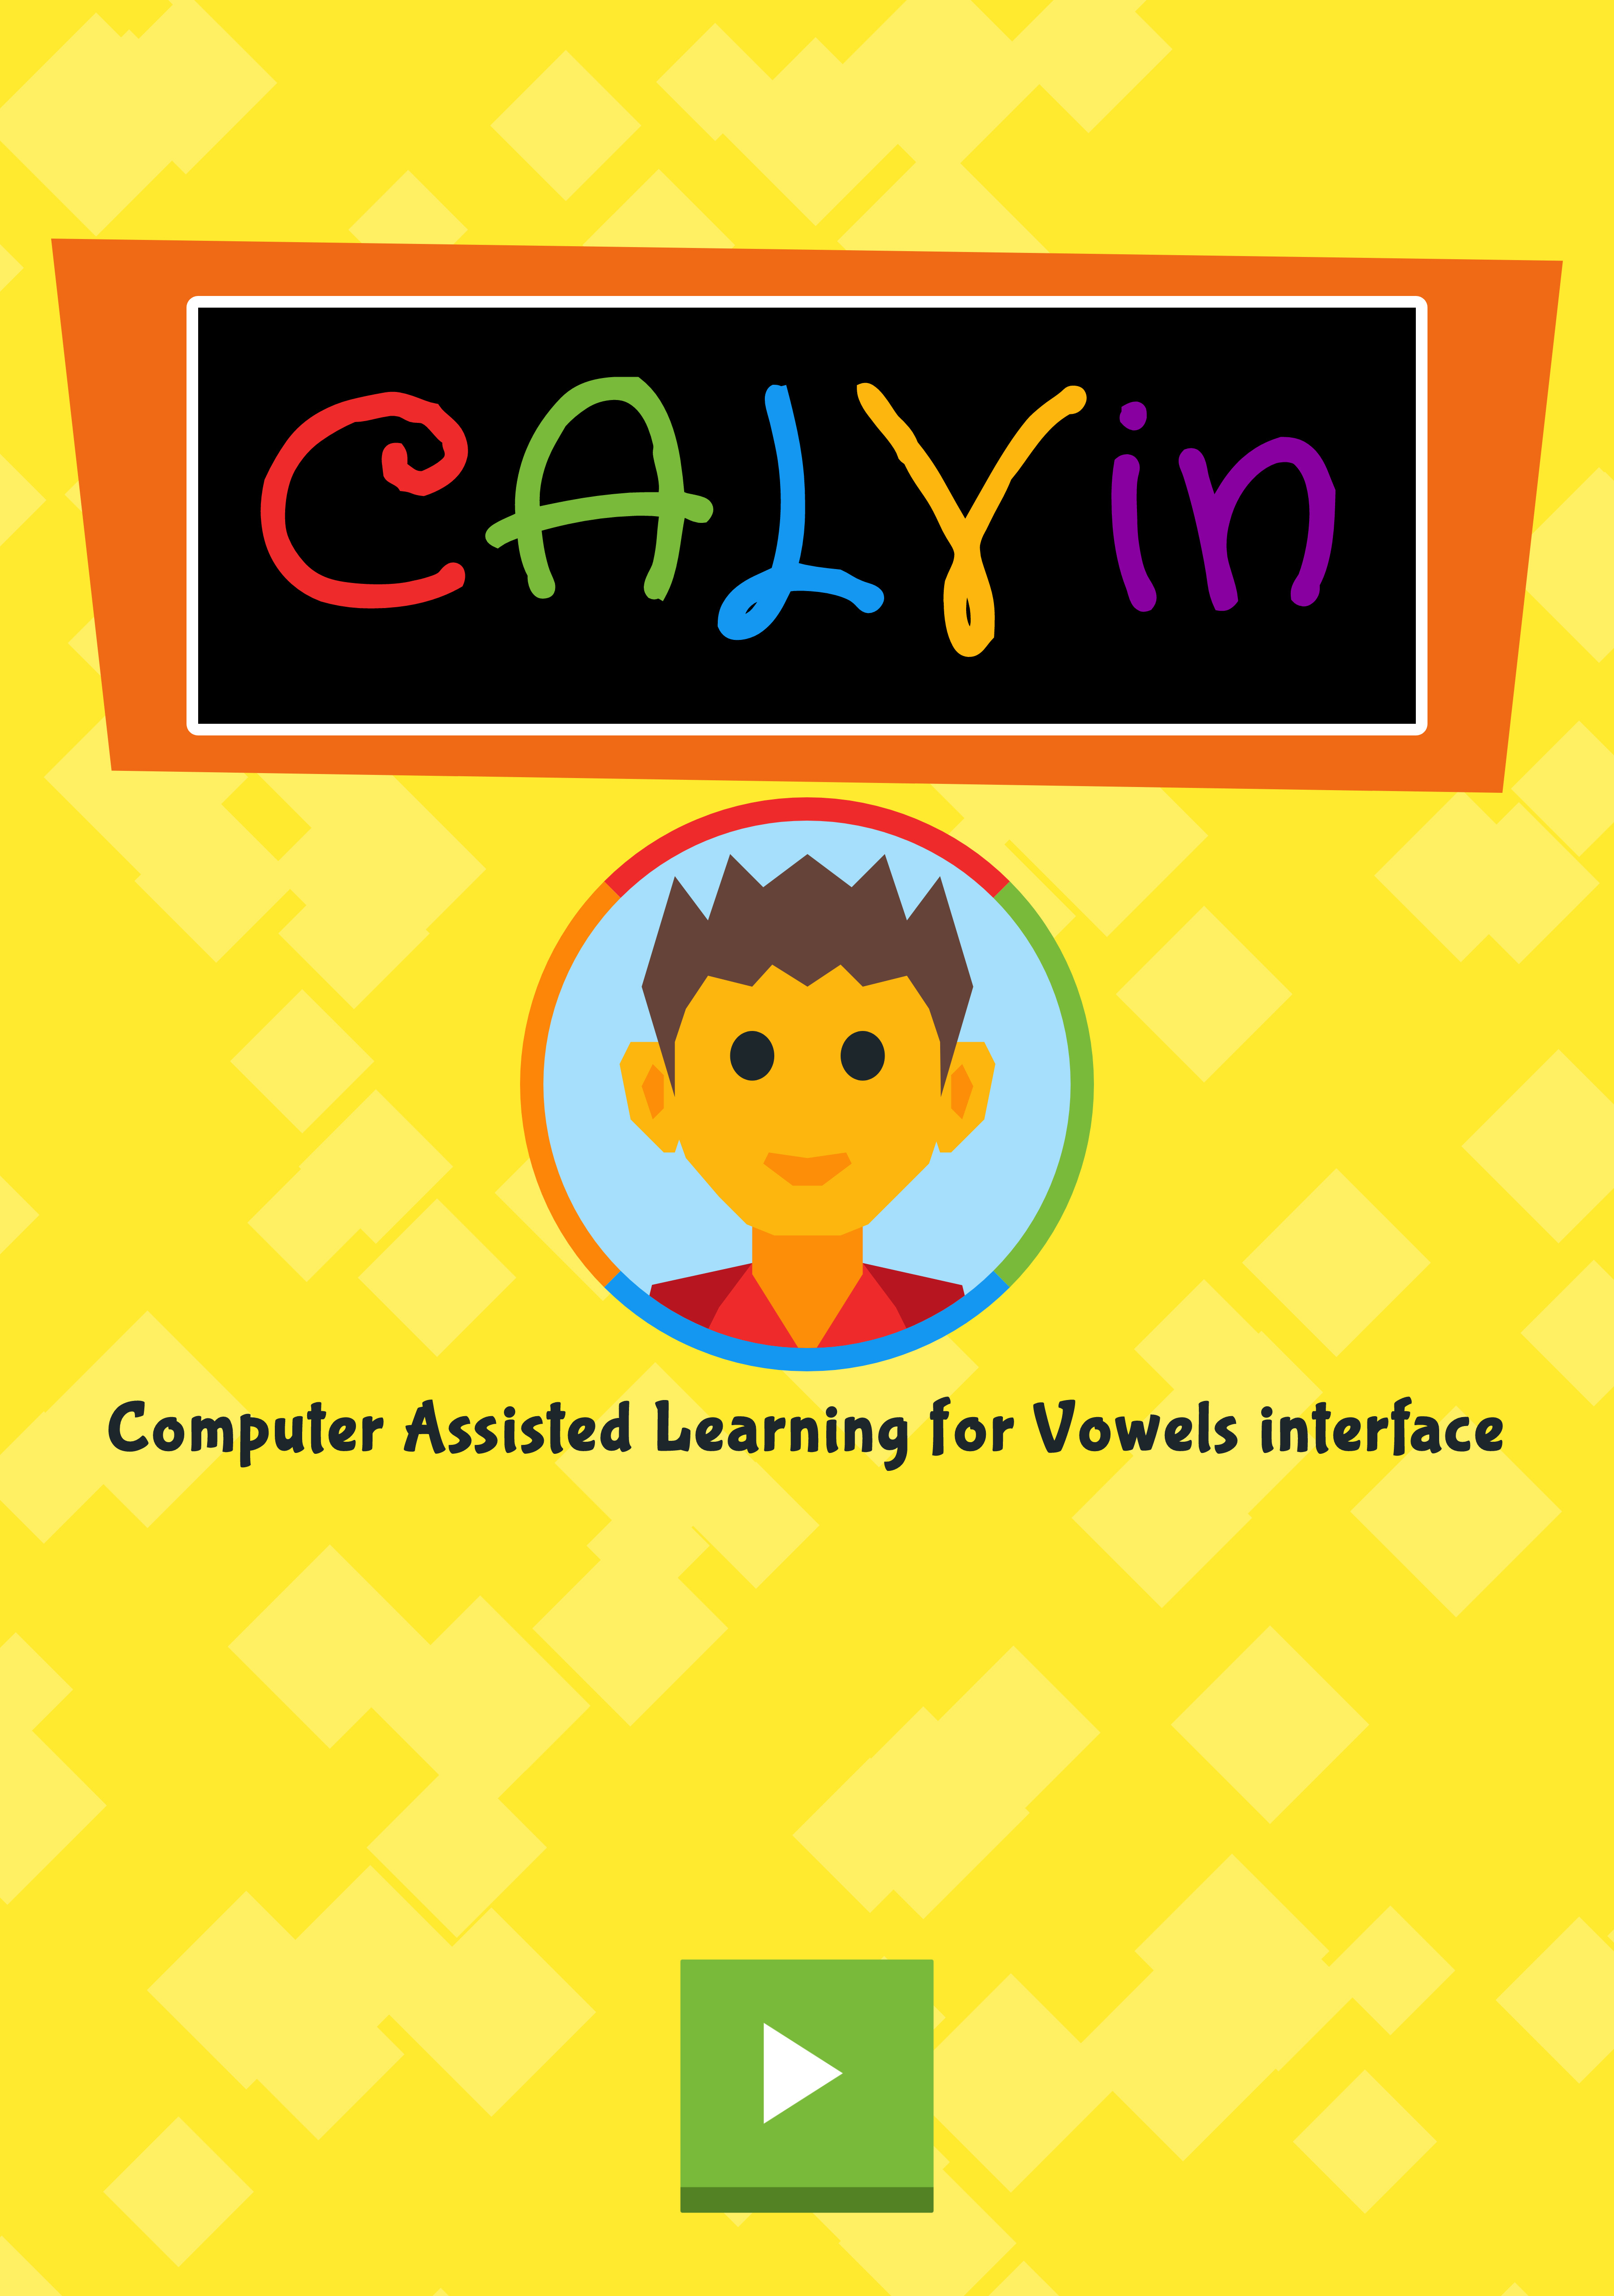
\includegraphics[width=\linewidth]{images/CALVin-screenshots/jpgs/calvin_start}
  \end{column}
  \begin{column}{\screenshotwidth}
    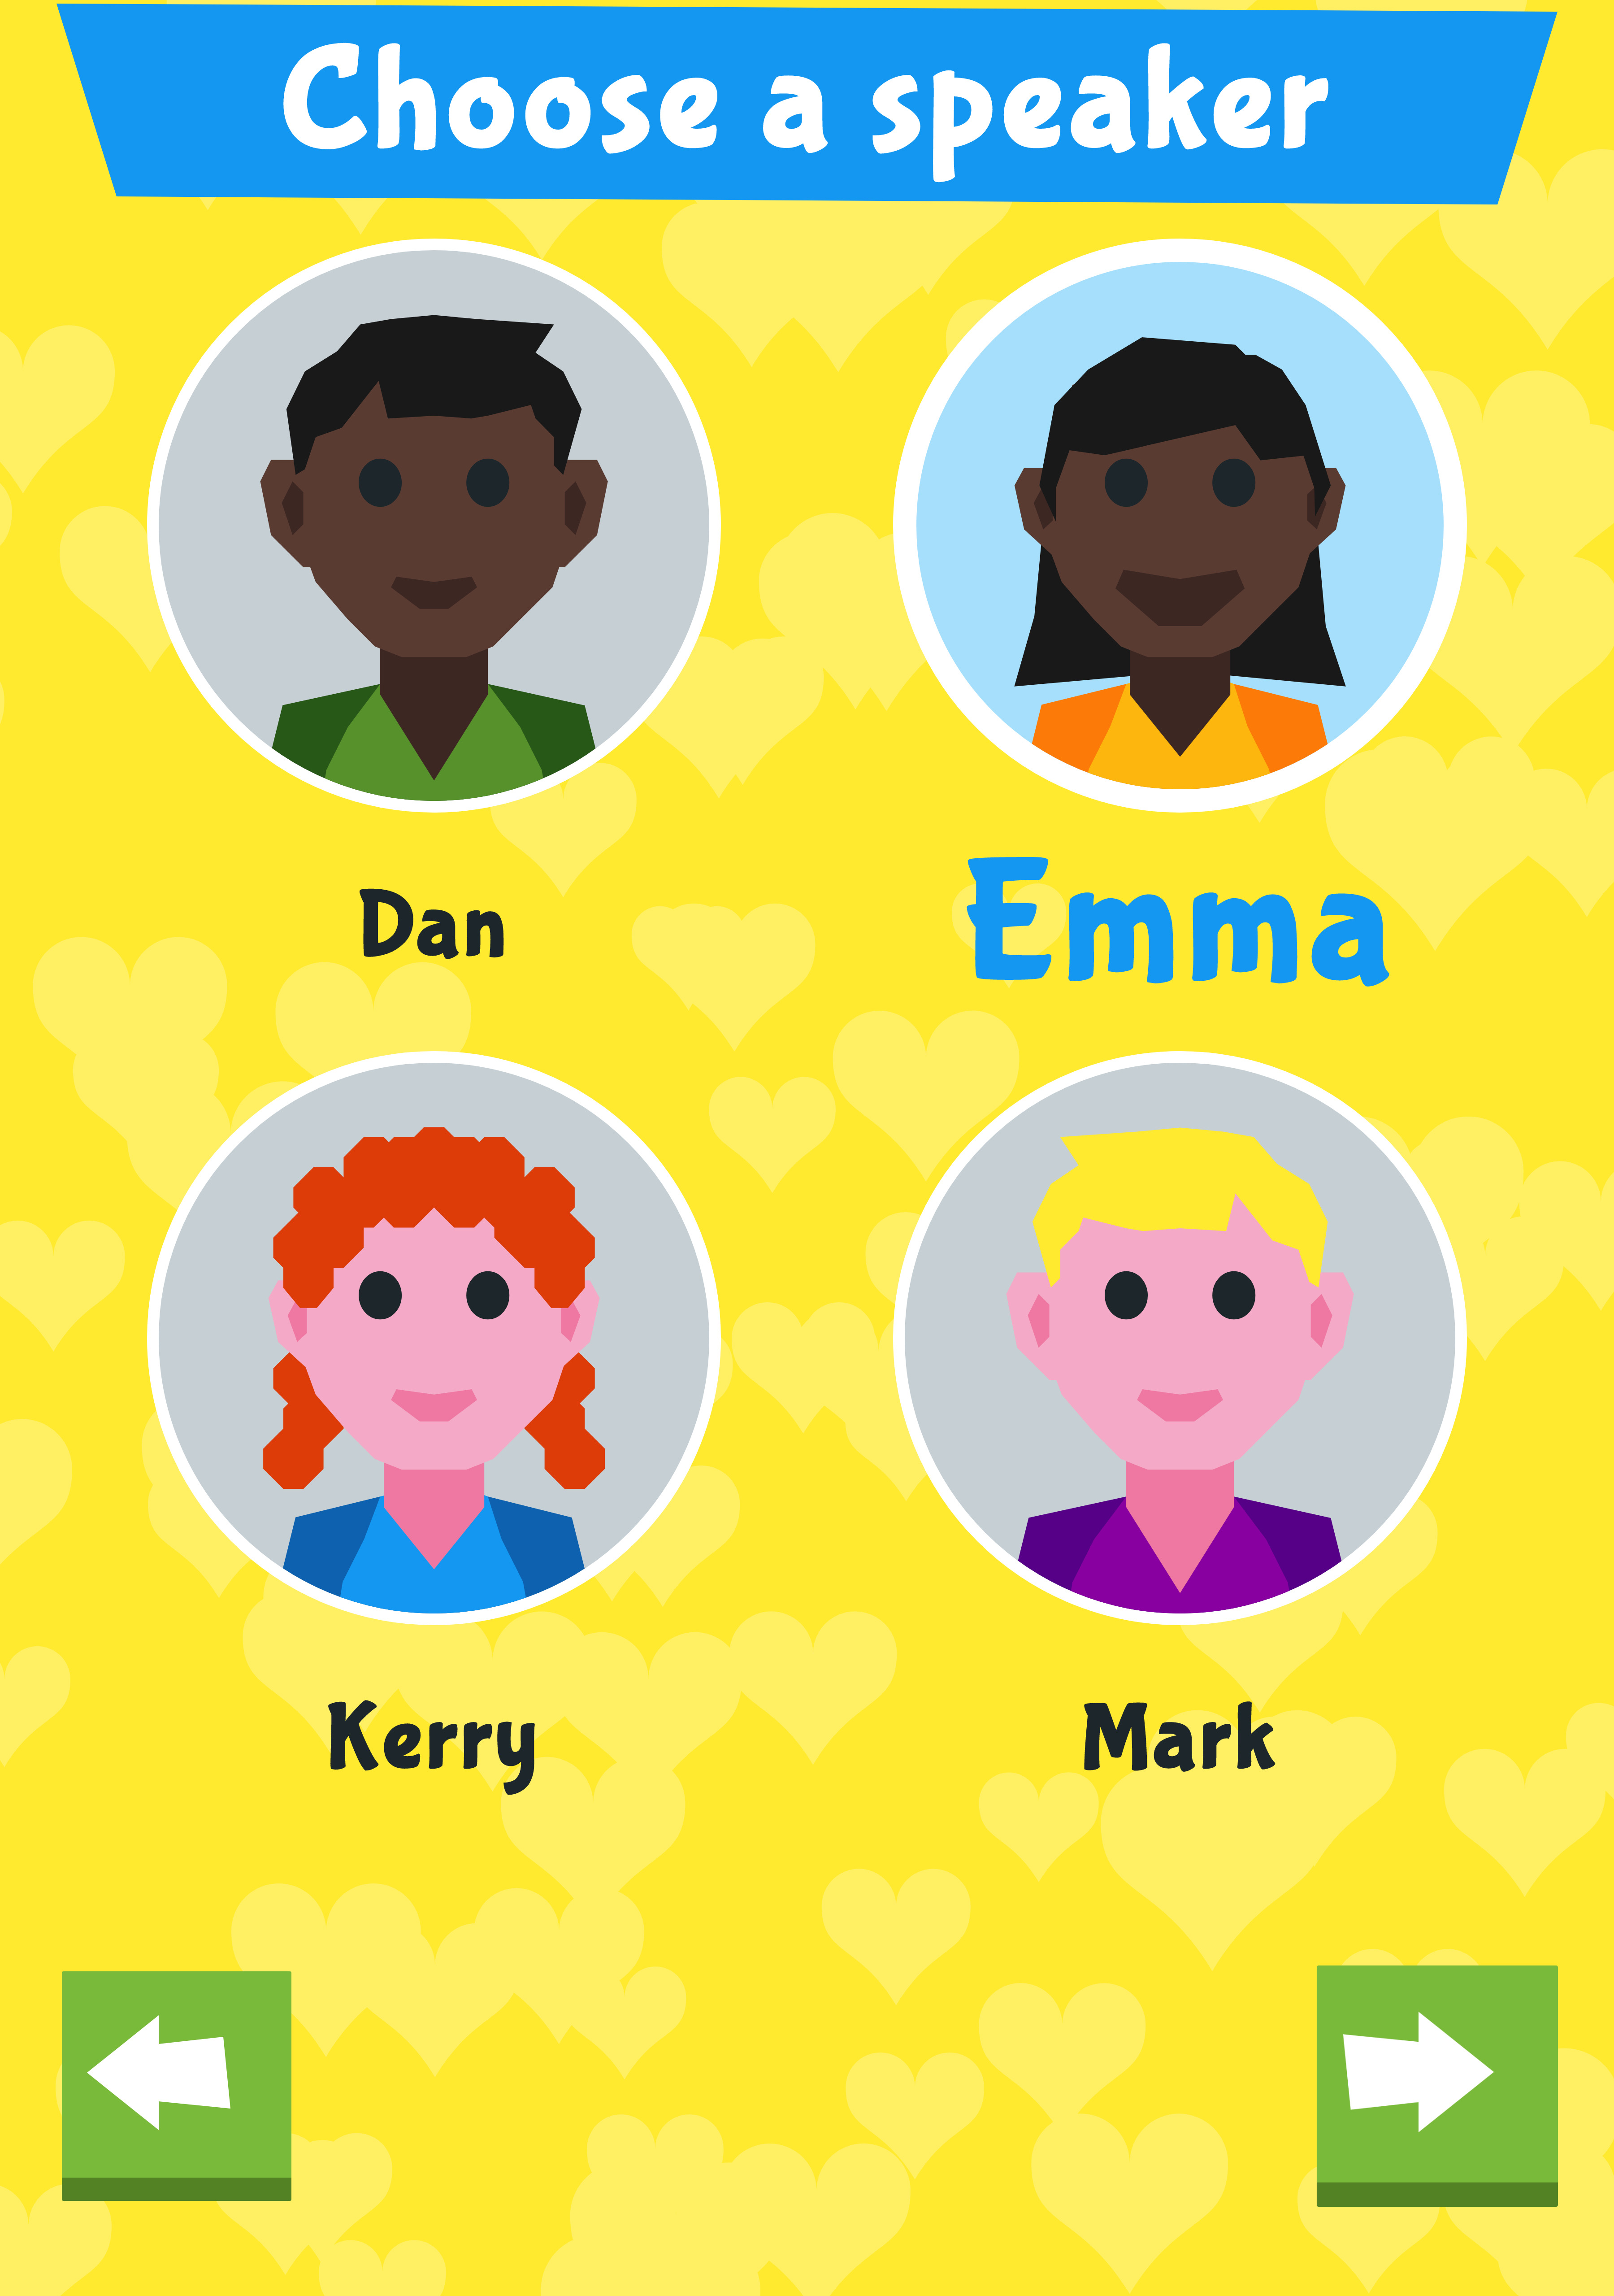
\includegraphics[width=\linewidth]{images/CALVin-screenshots/jpgs/choose_talker}
  \end{column}
  \begin{column}{\screenshotwidth}
    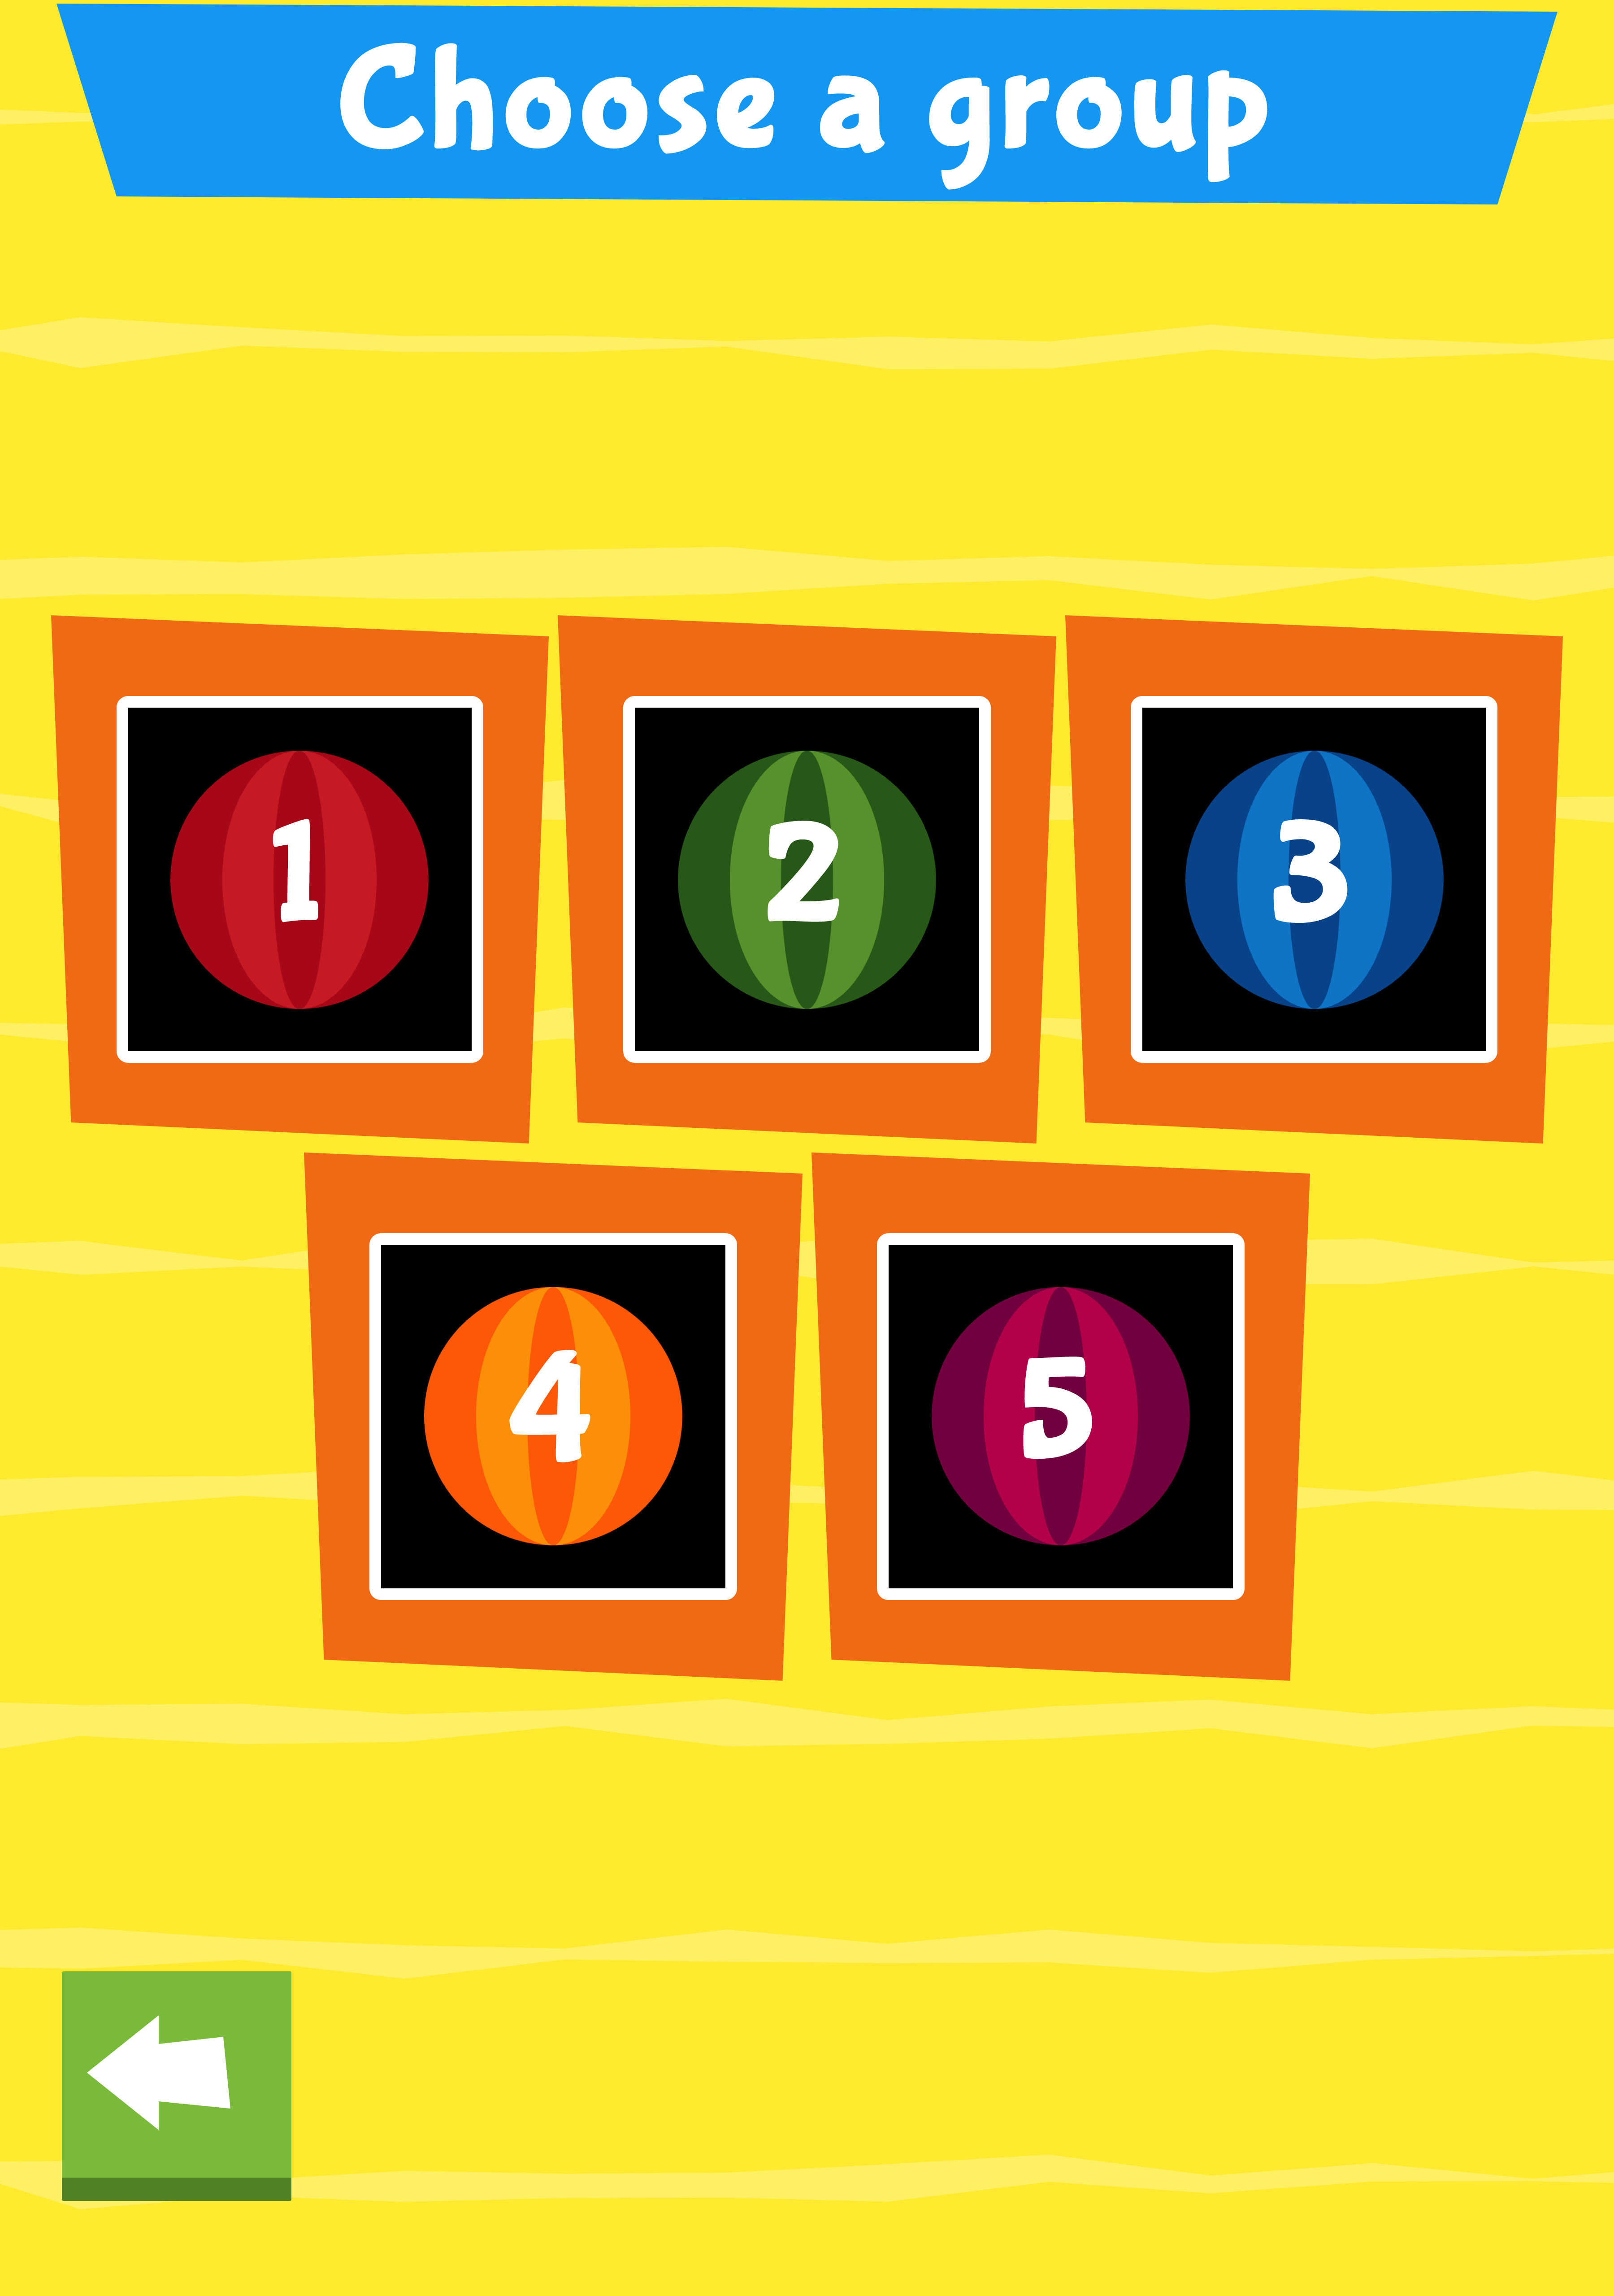
\includegraphics[width=\linewidth]{images/CALVin-screenshots/jpgs/choose_group}
  \end{column}
  \begin{column}{\screenshotwidth}
    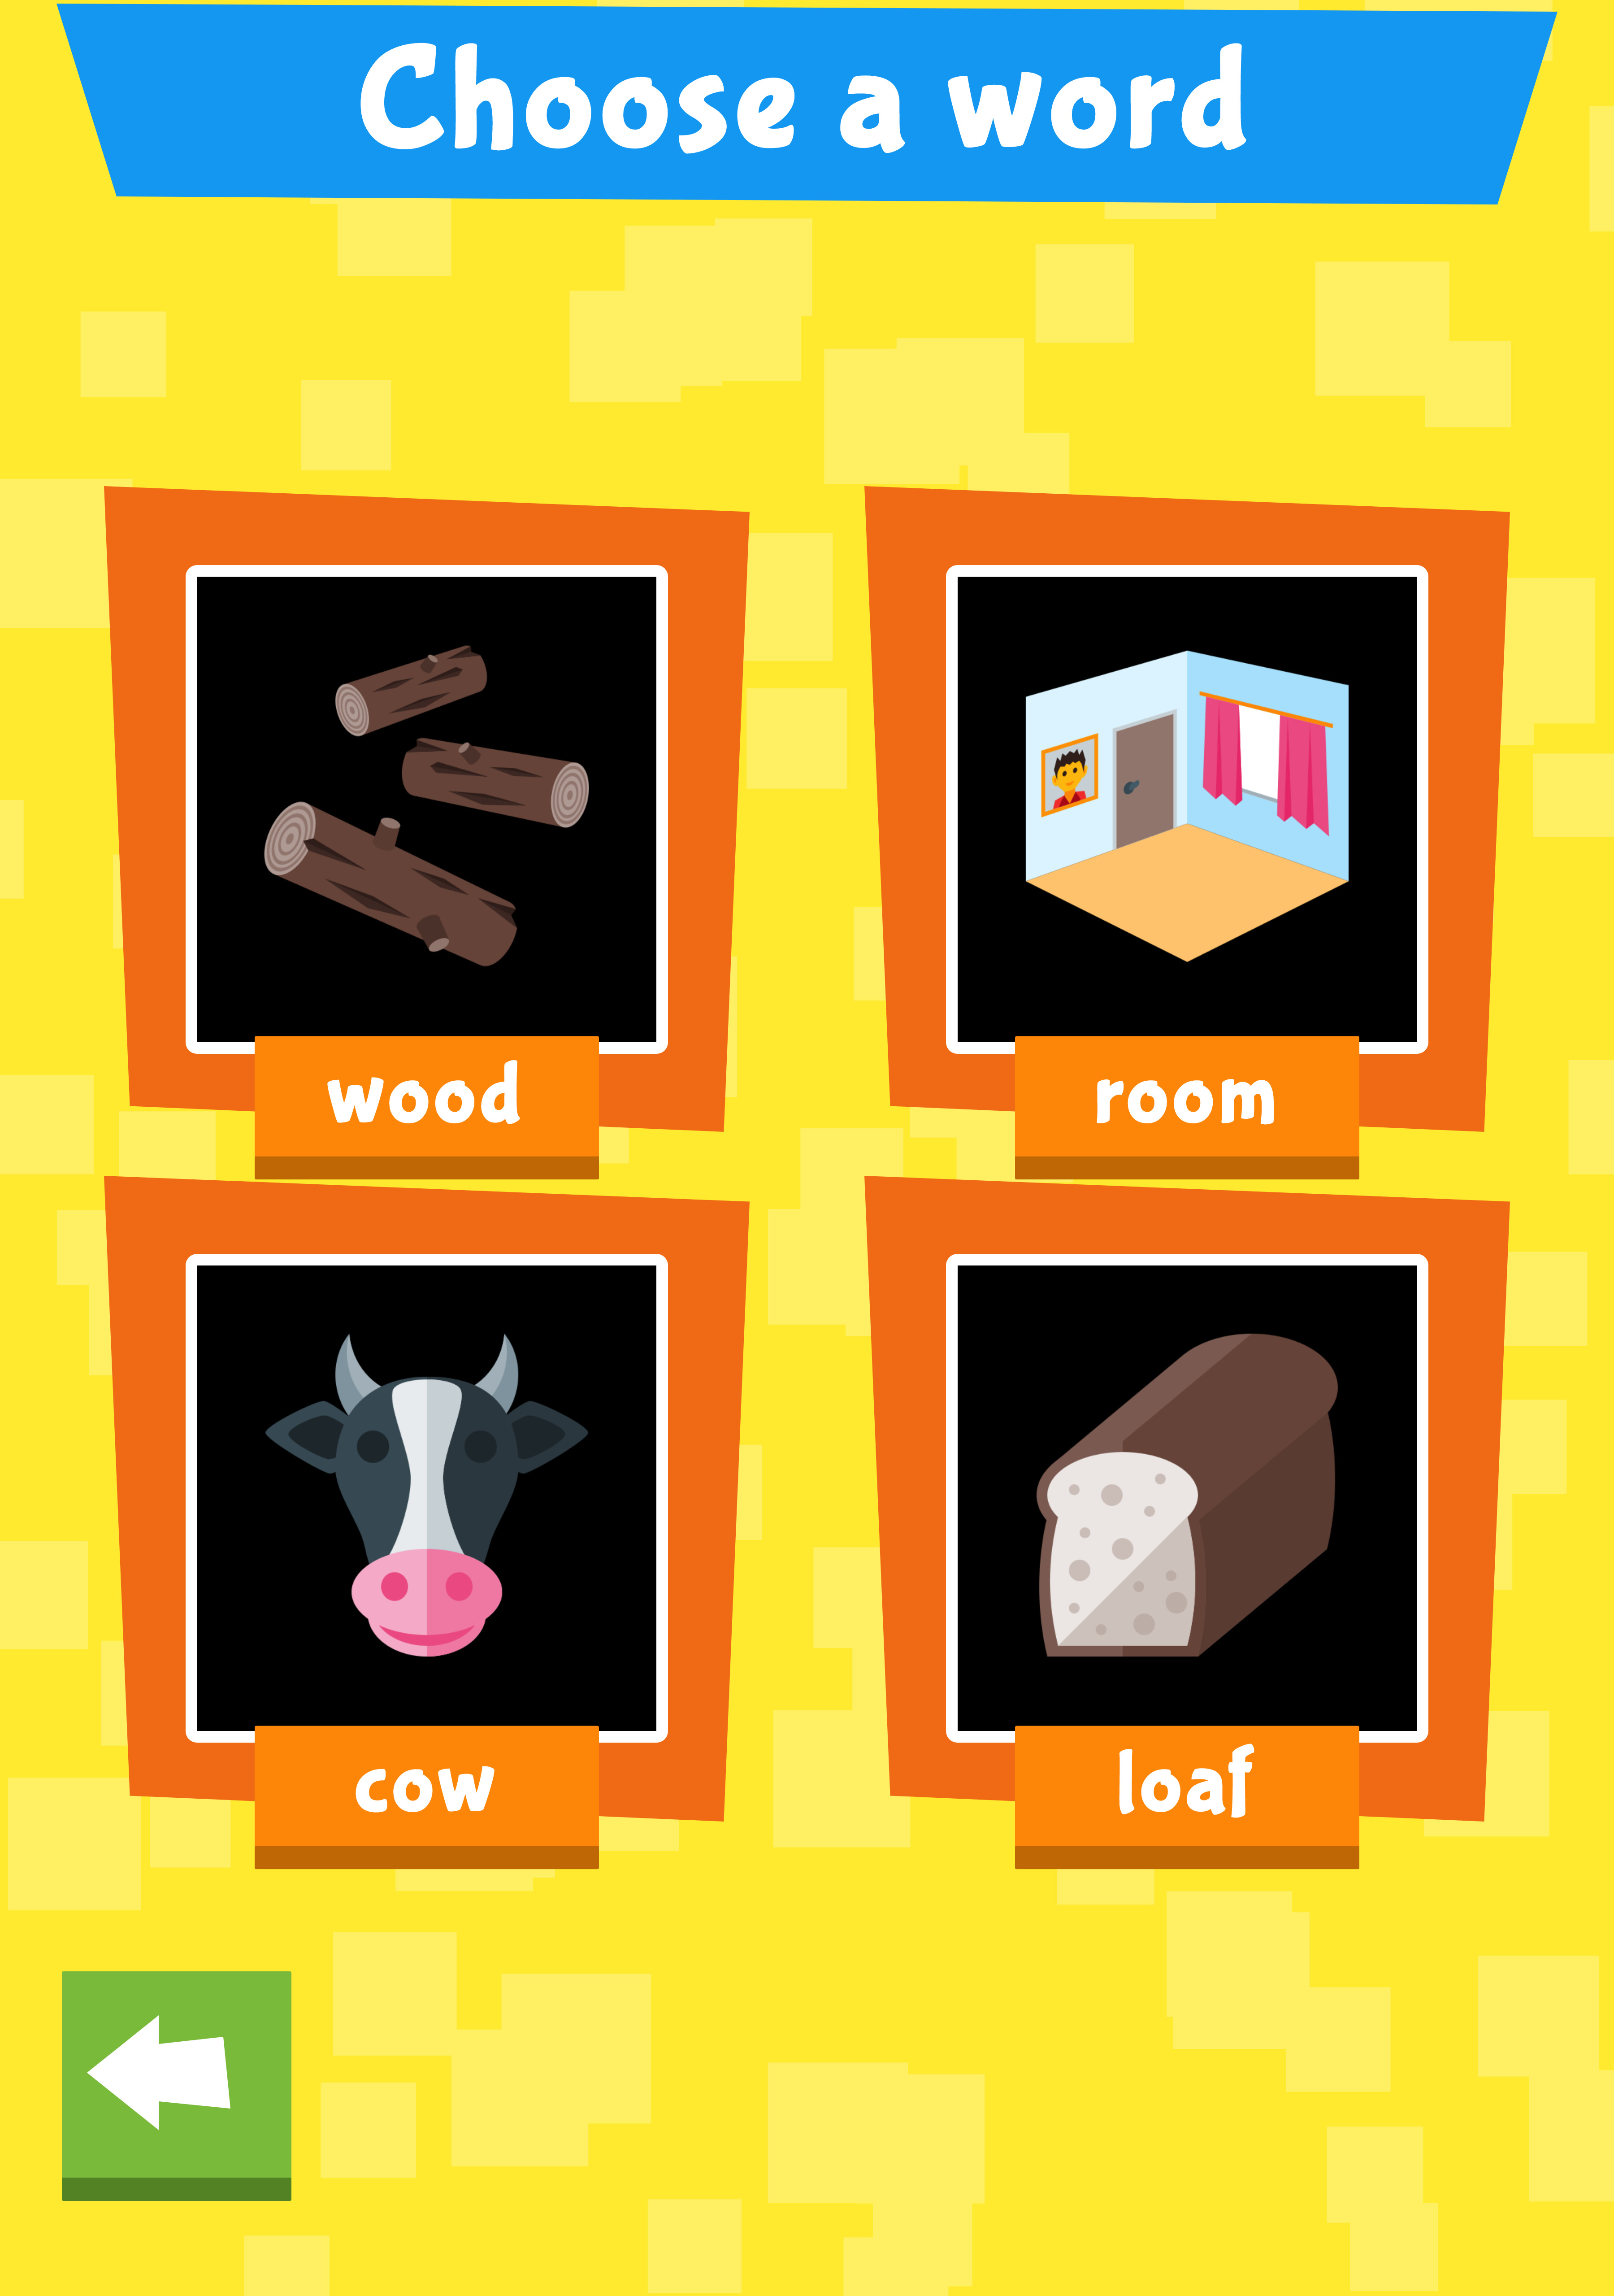
\includegraphics[width=\linewidth]{images/CALVin-screenshots/jpgs/choose_word}
  \end{column}
\end{columns}
\vspace*{1ex}
\begin{columns}
  \begin{column}{\screenshotwidth}
    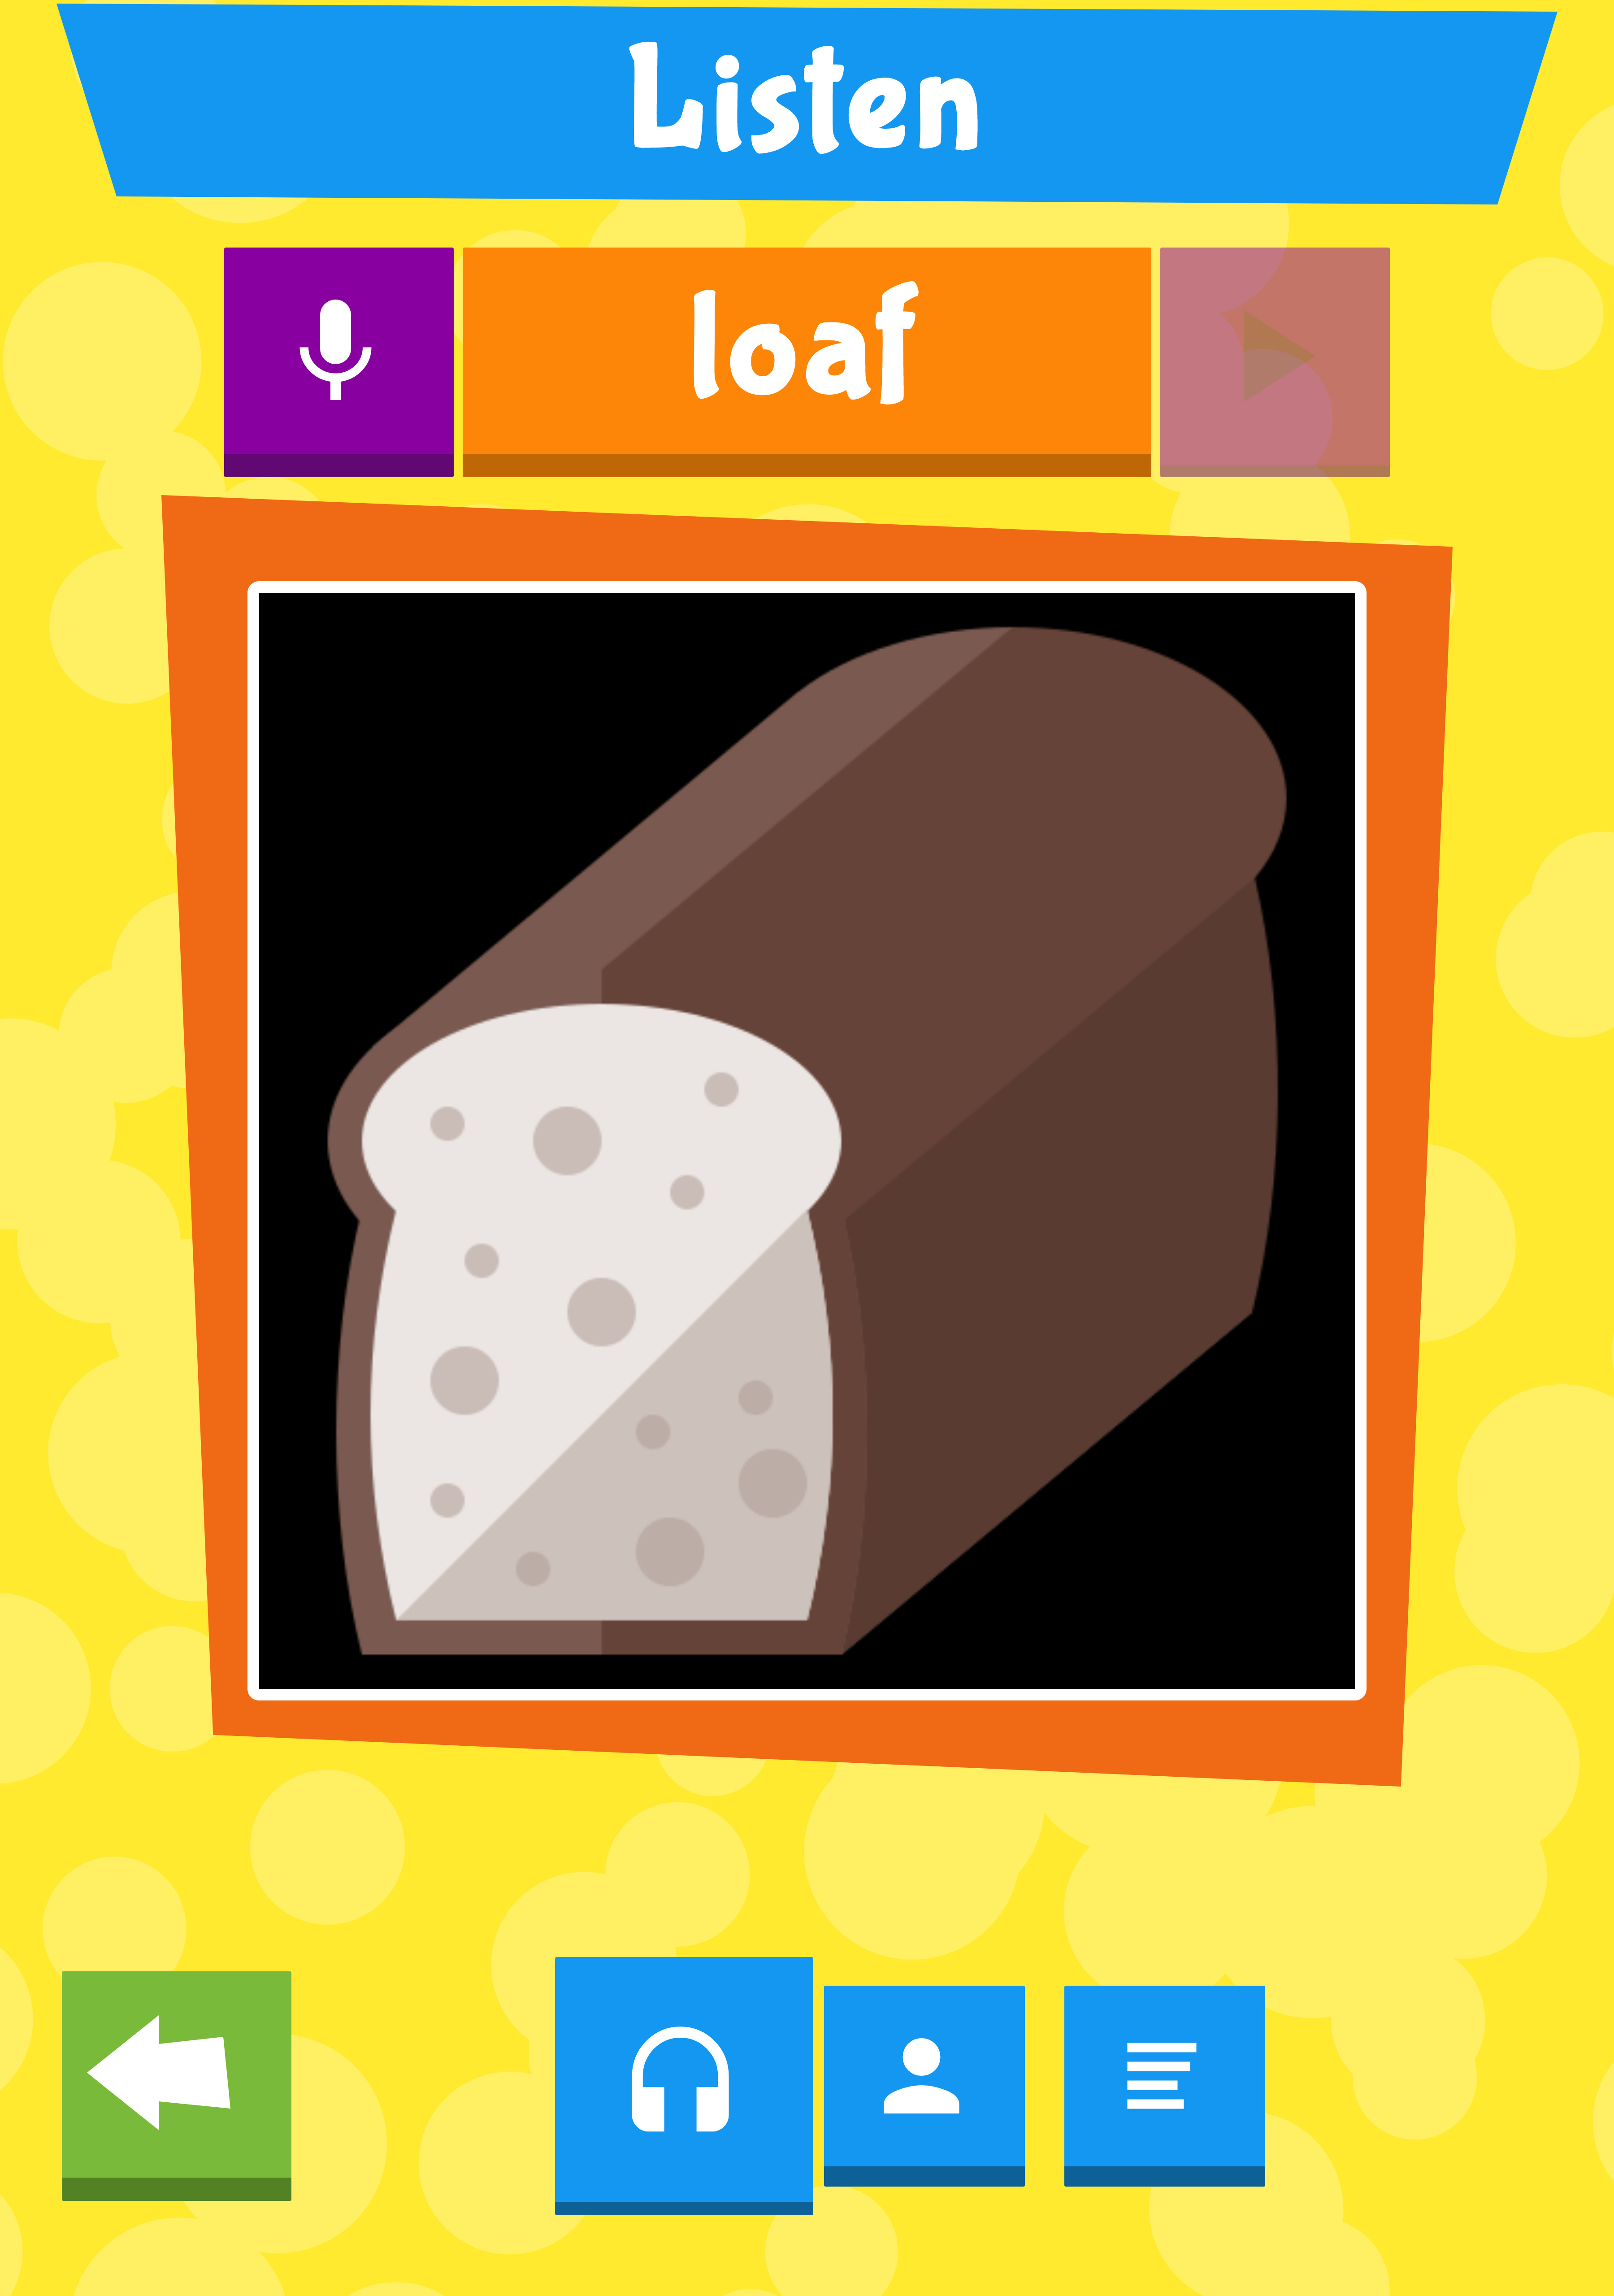
\includegraphics[width=\linewidth]{images/CALVin-screenshots/jpgs/word}
  \end{column}
  \begin{column}{\screenshotwidth}
    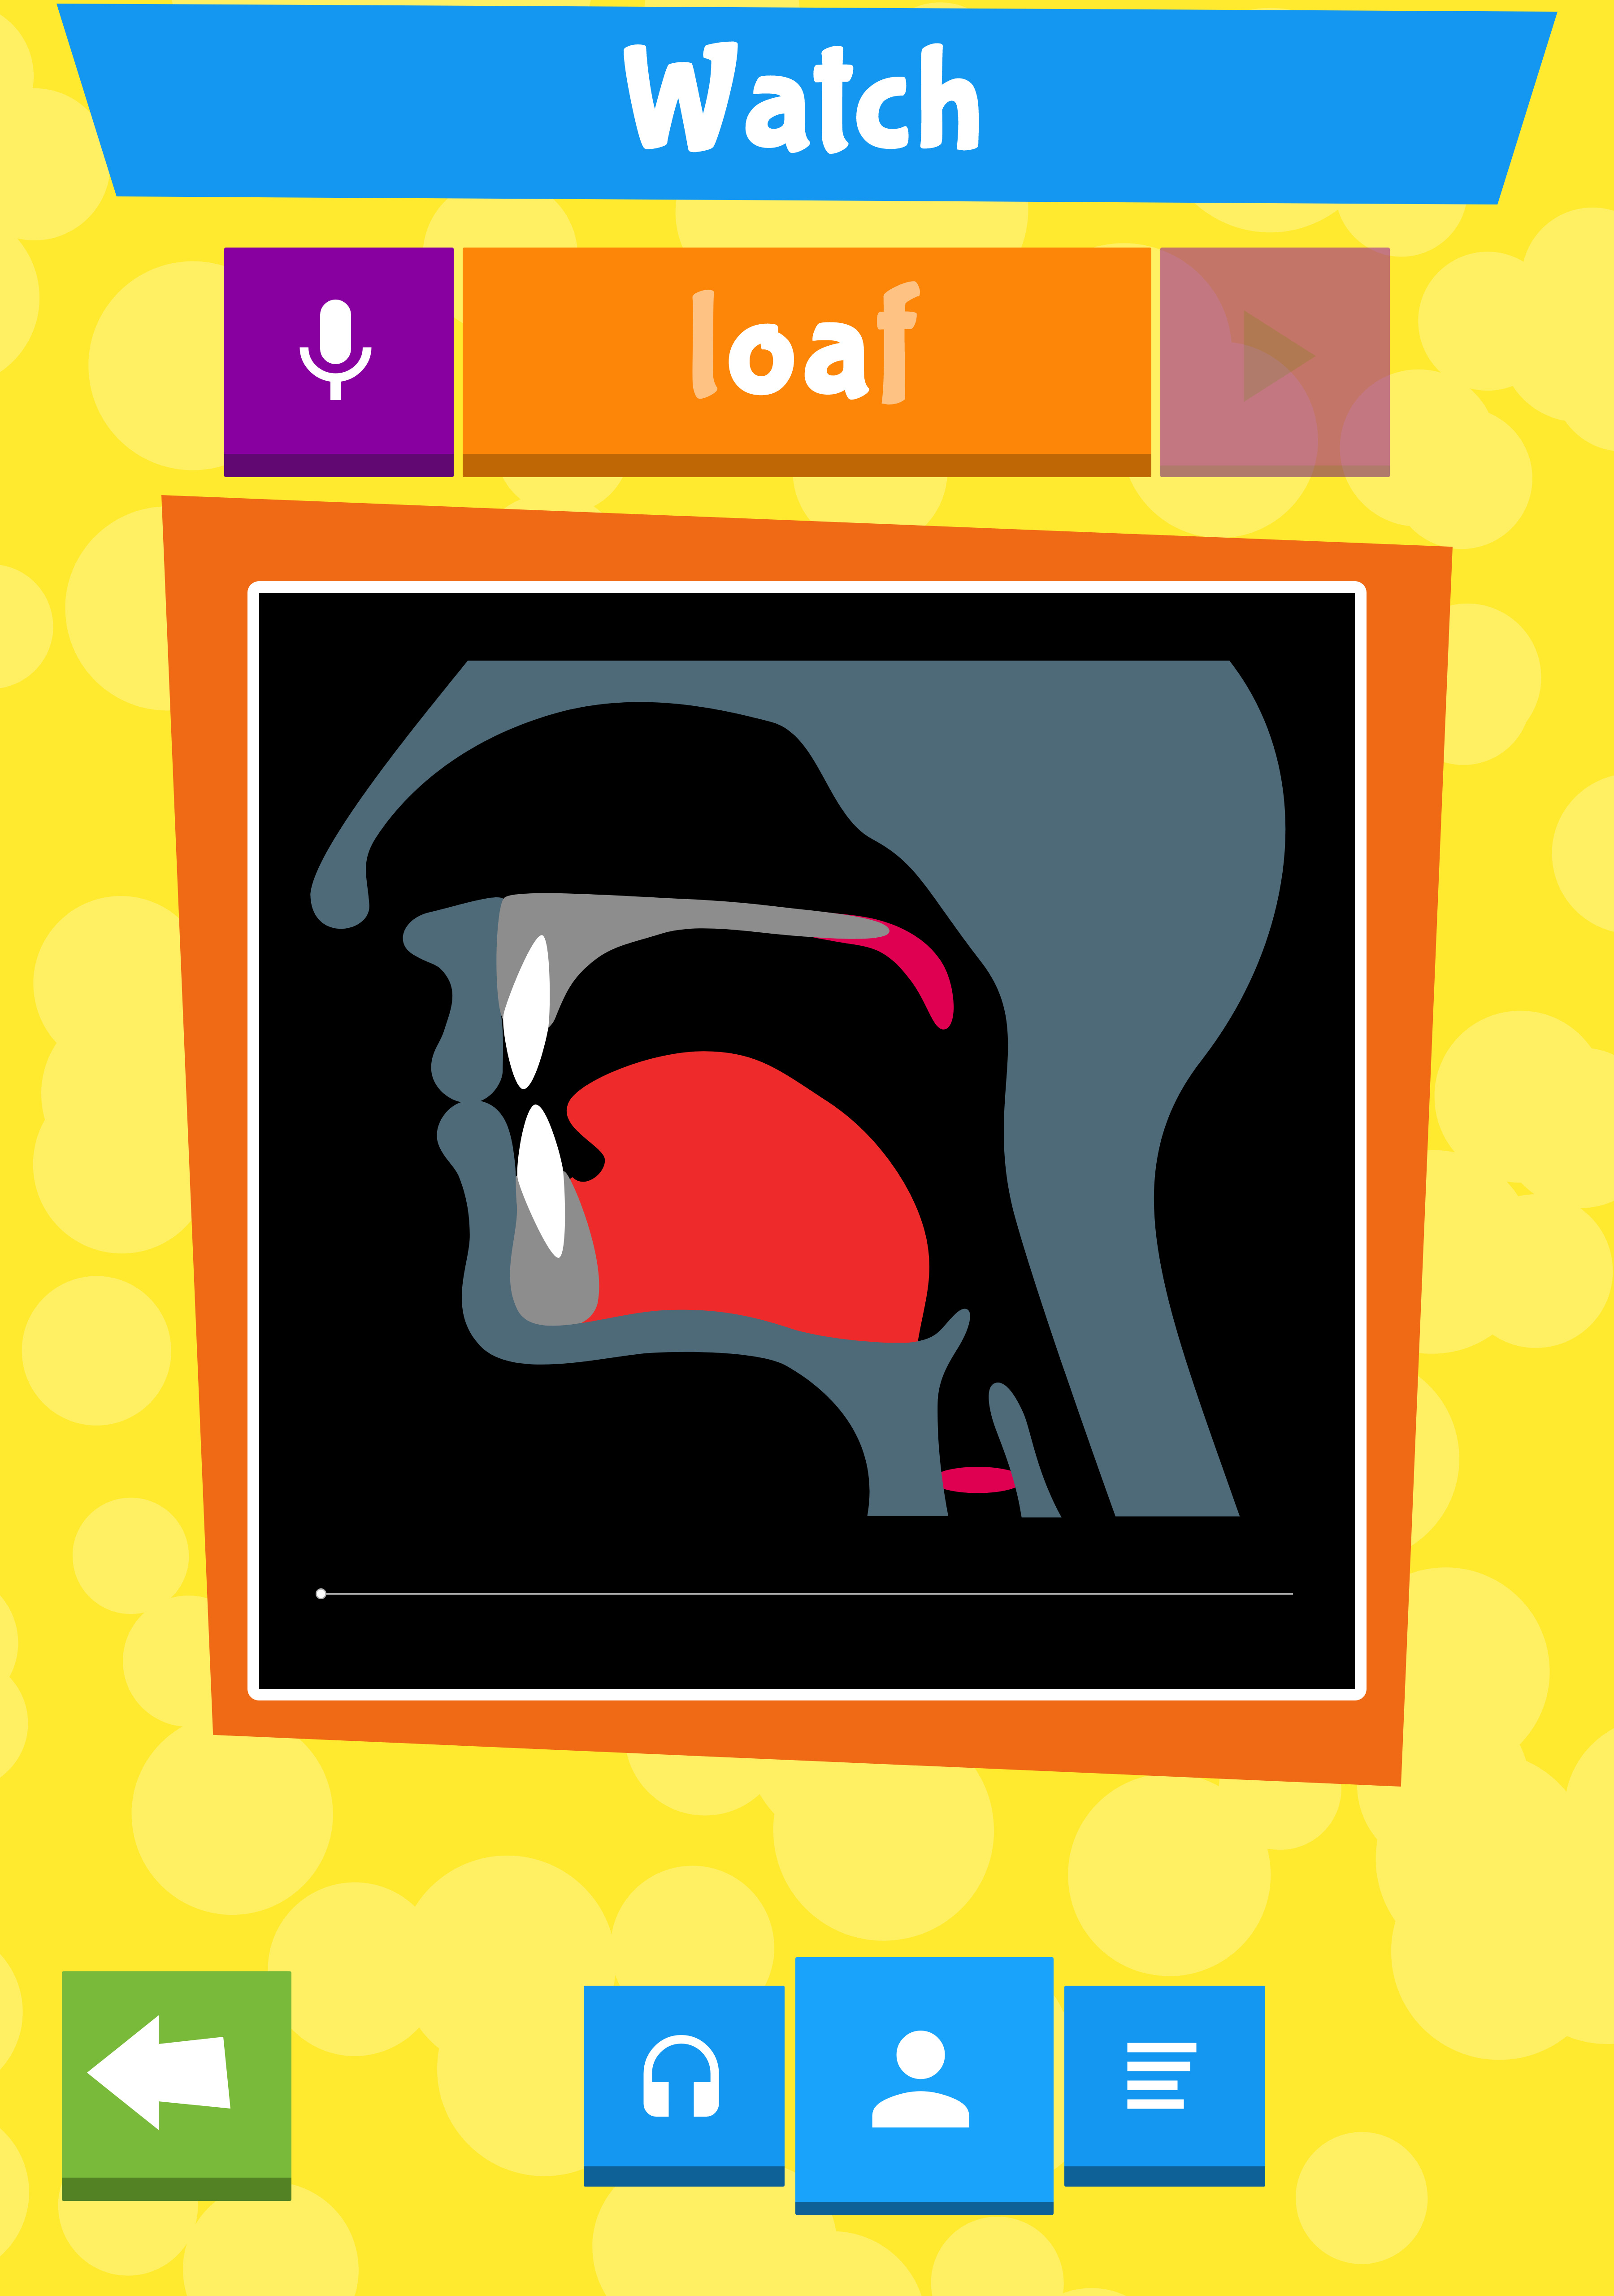
\includegraphics[width=\linewidth]{images/CALVin-screenshots/jpgs/vocal_tract_animation}
  \end{column}
  \begin{column}{\screenshotwidth}
    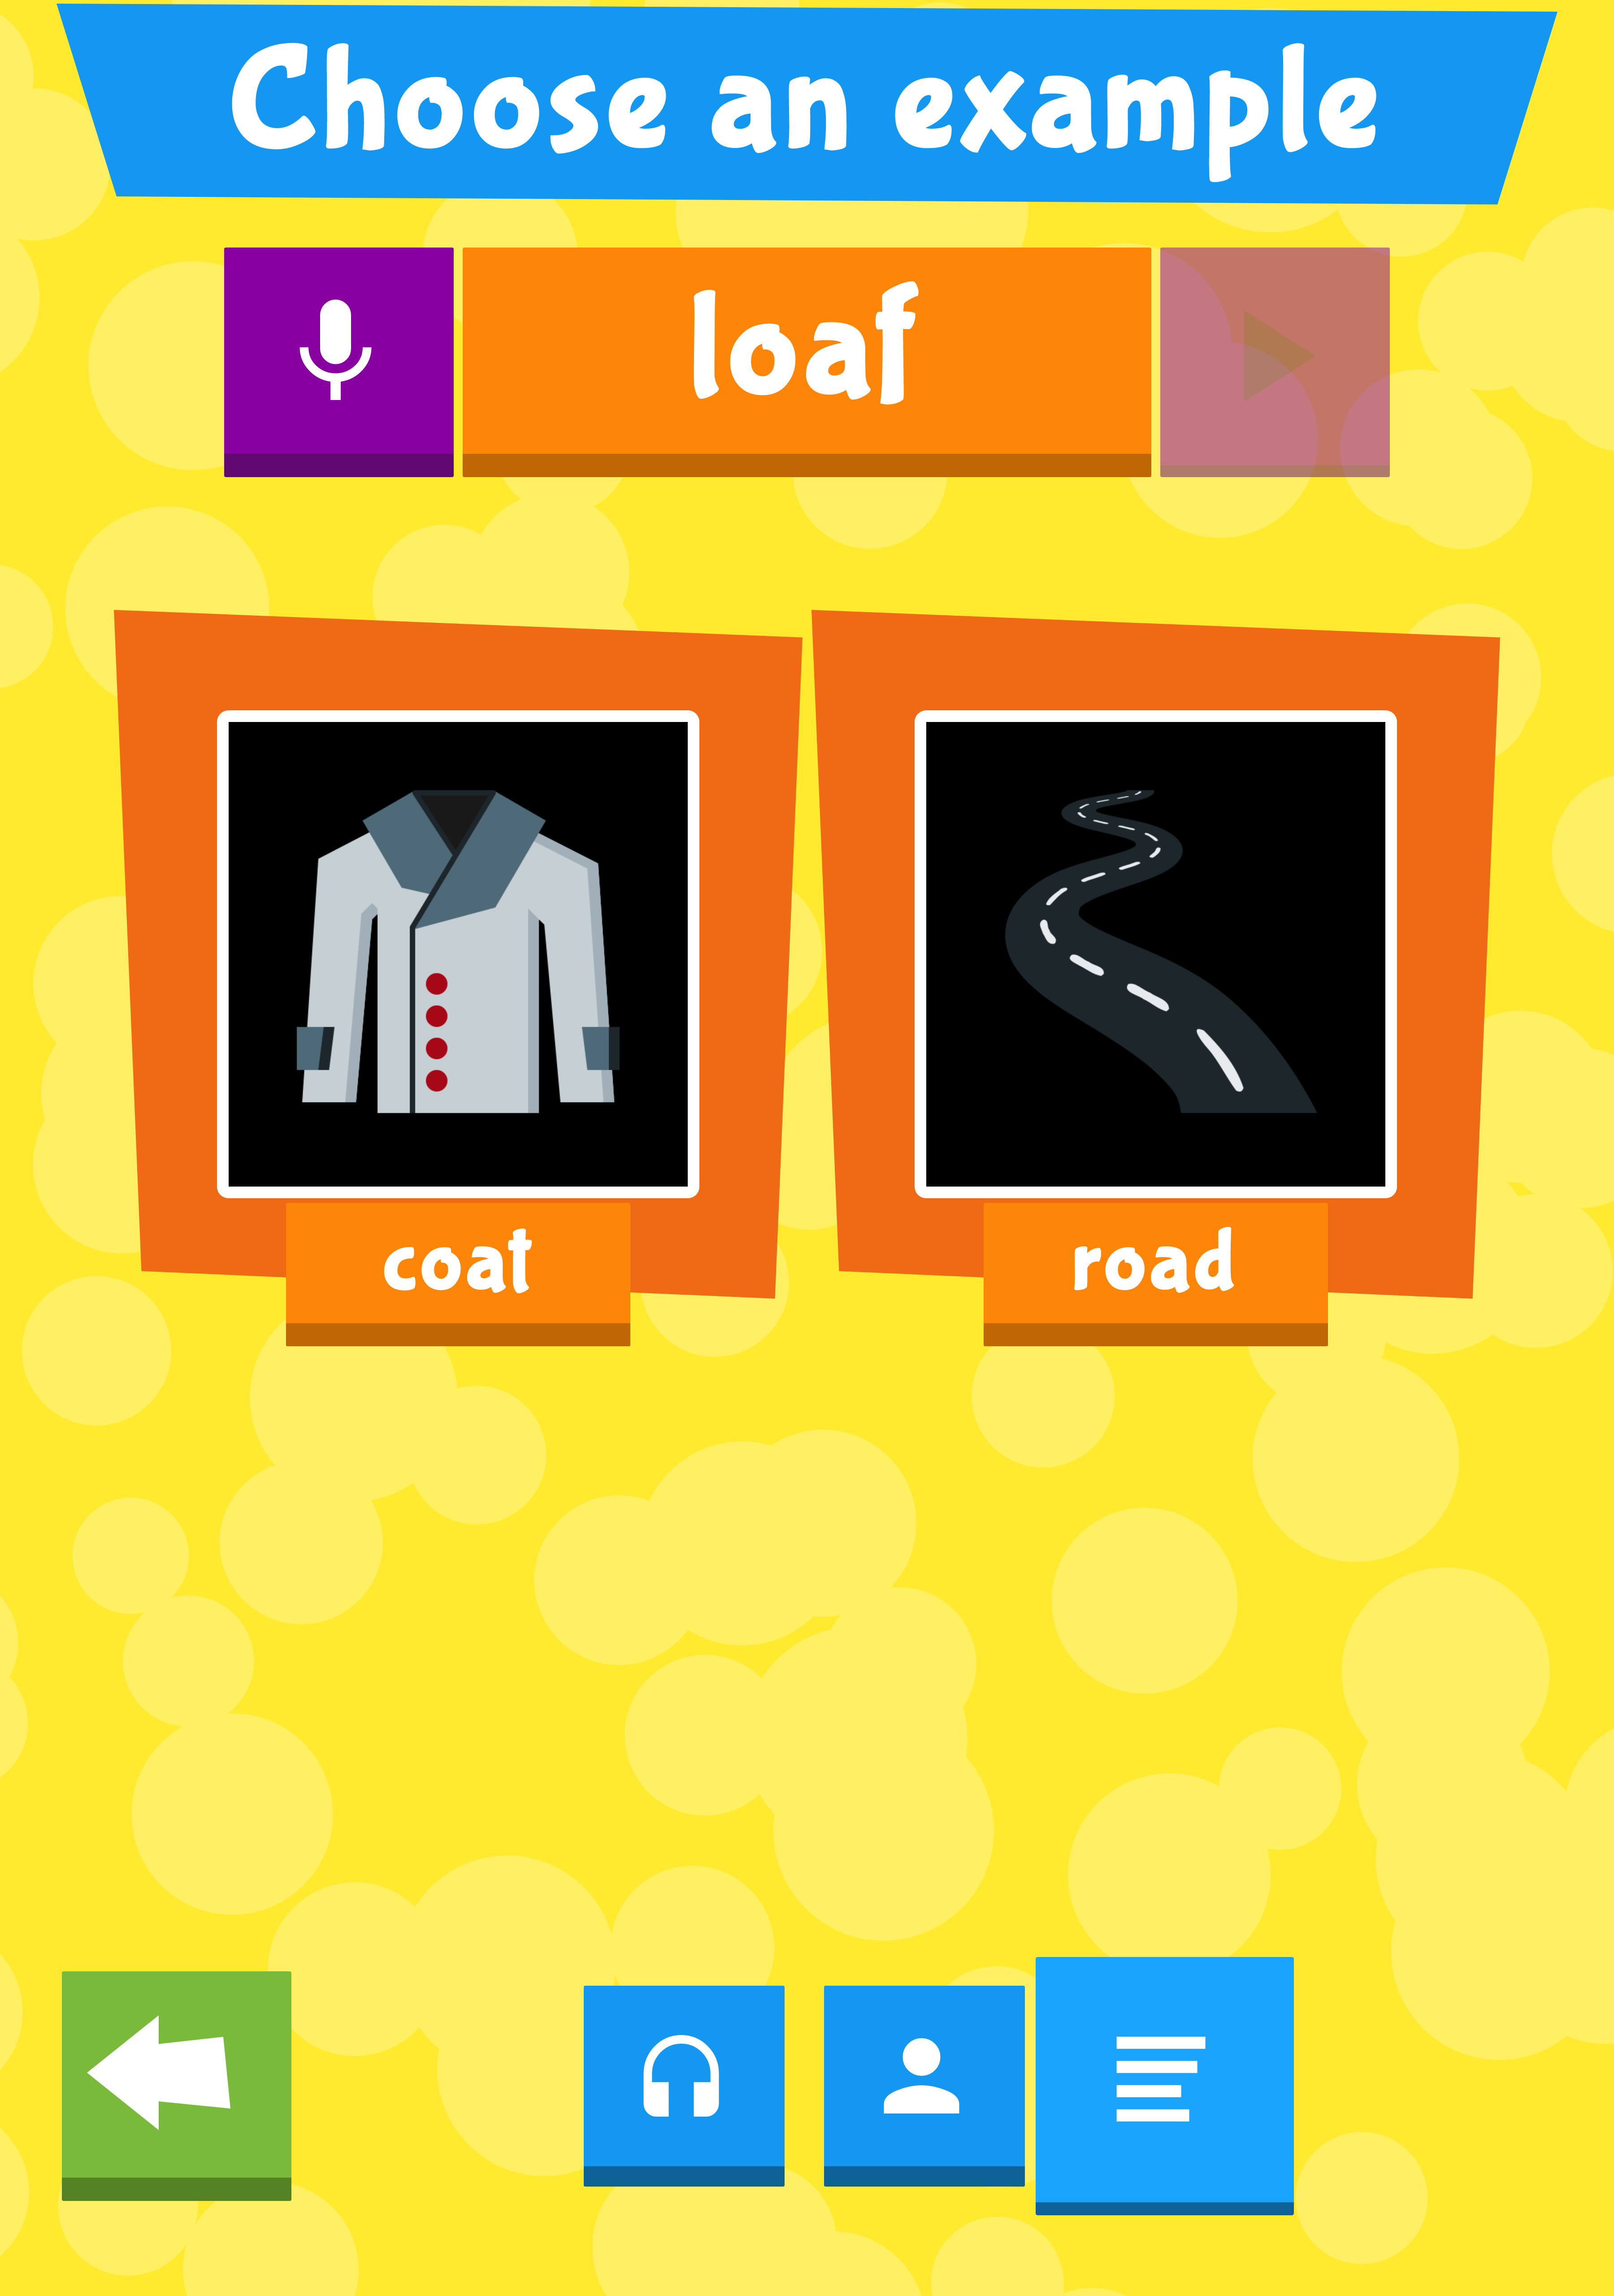
\includegraphics[width=\linewidth]{images/CALVin-screenshots/jpgs/choose_example}
  \end{column}
  \begin{column}{\screenshotwidth}
    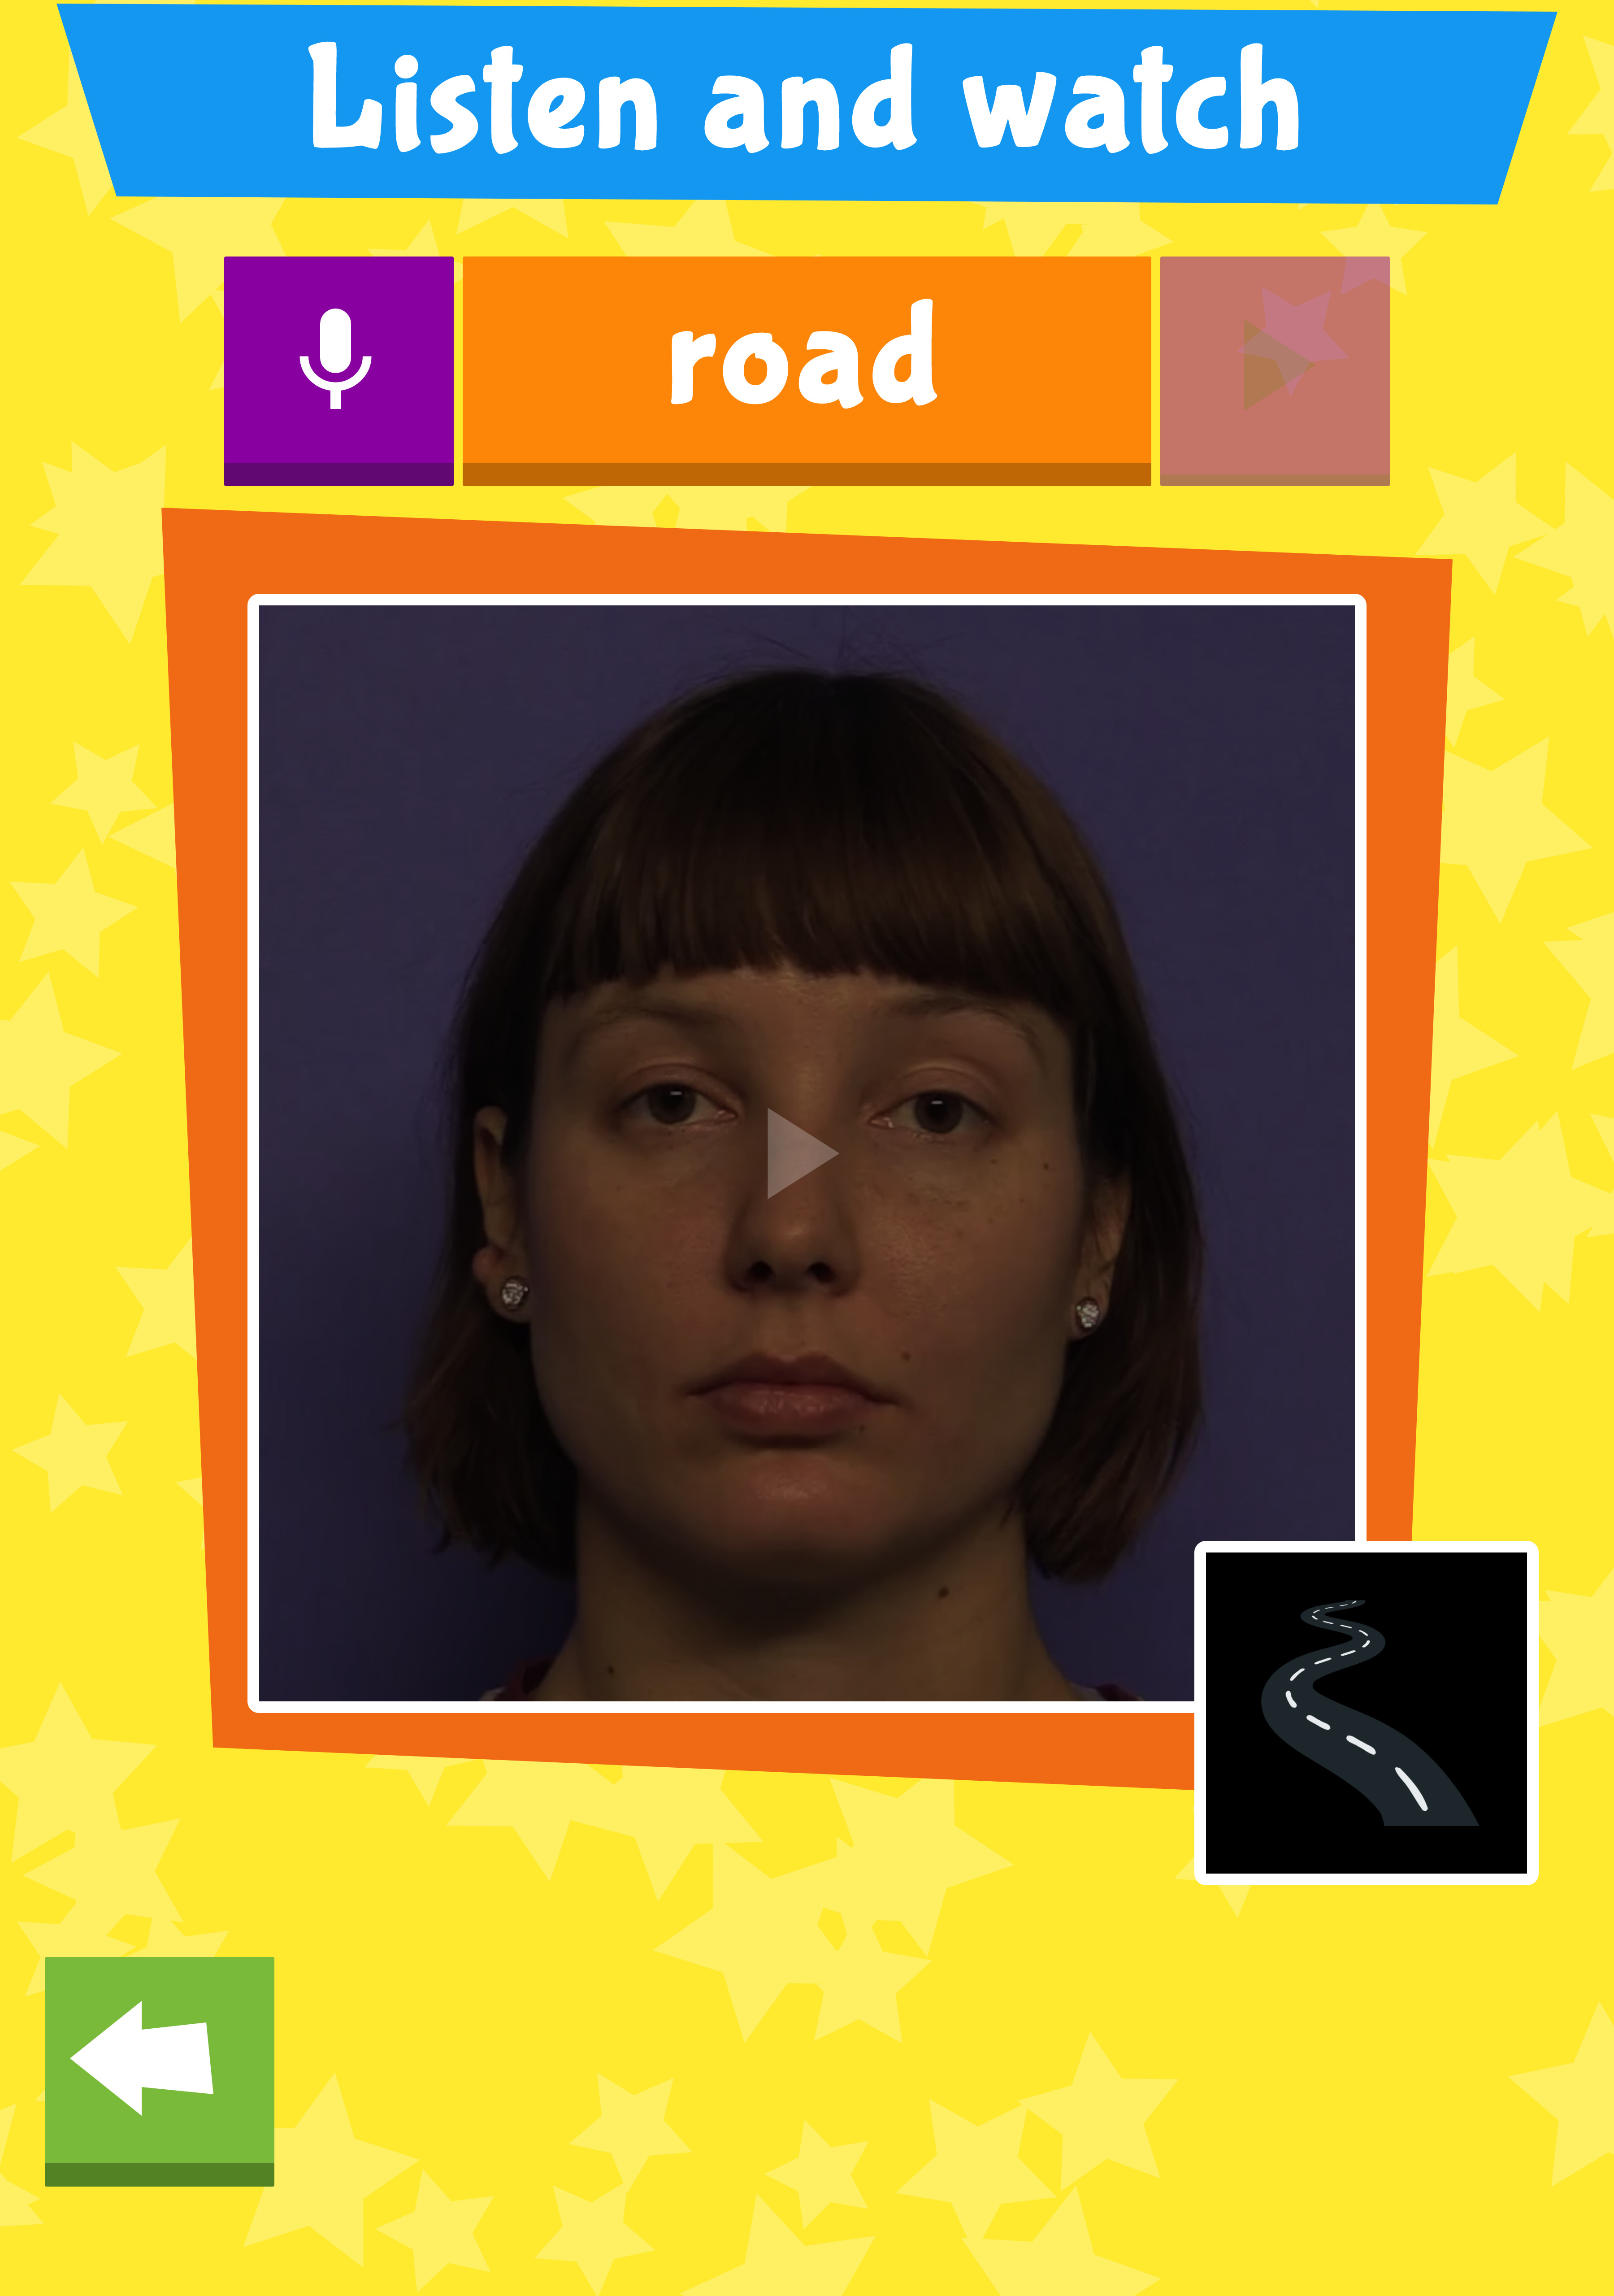
\includegraphics[width=\linewidth]{images/CALVin-screenshots/jpgs/watch_example}
  \end{column}
\end{columns}
\vspace*{1ex}
\caption{Screenshots from CALVin}
\end{figure}
\end{block}

\end{column}
\begin{column}{0.5\linewidth}
\begin{block}{Results}
\paragraph{Perception (category discrimination)}

\vspace*{0.25in}
\begin{figure}
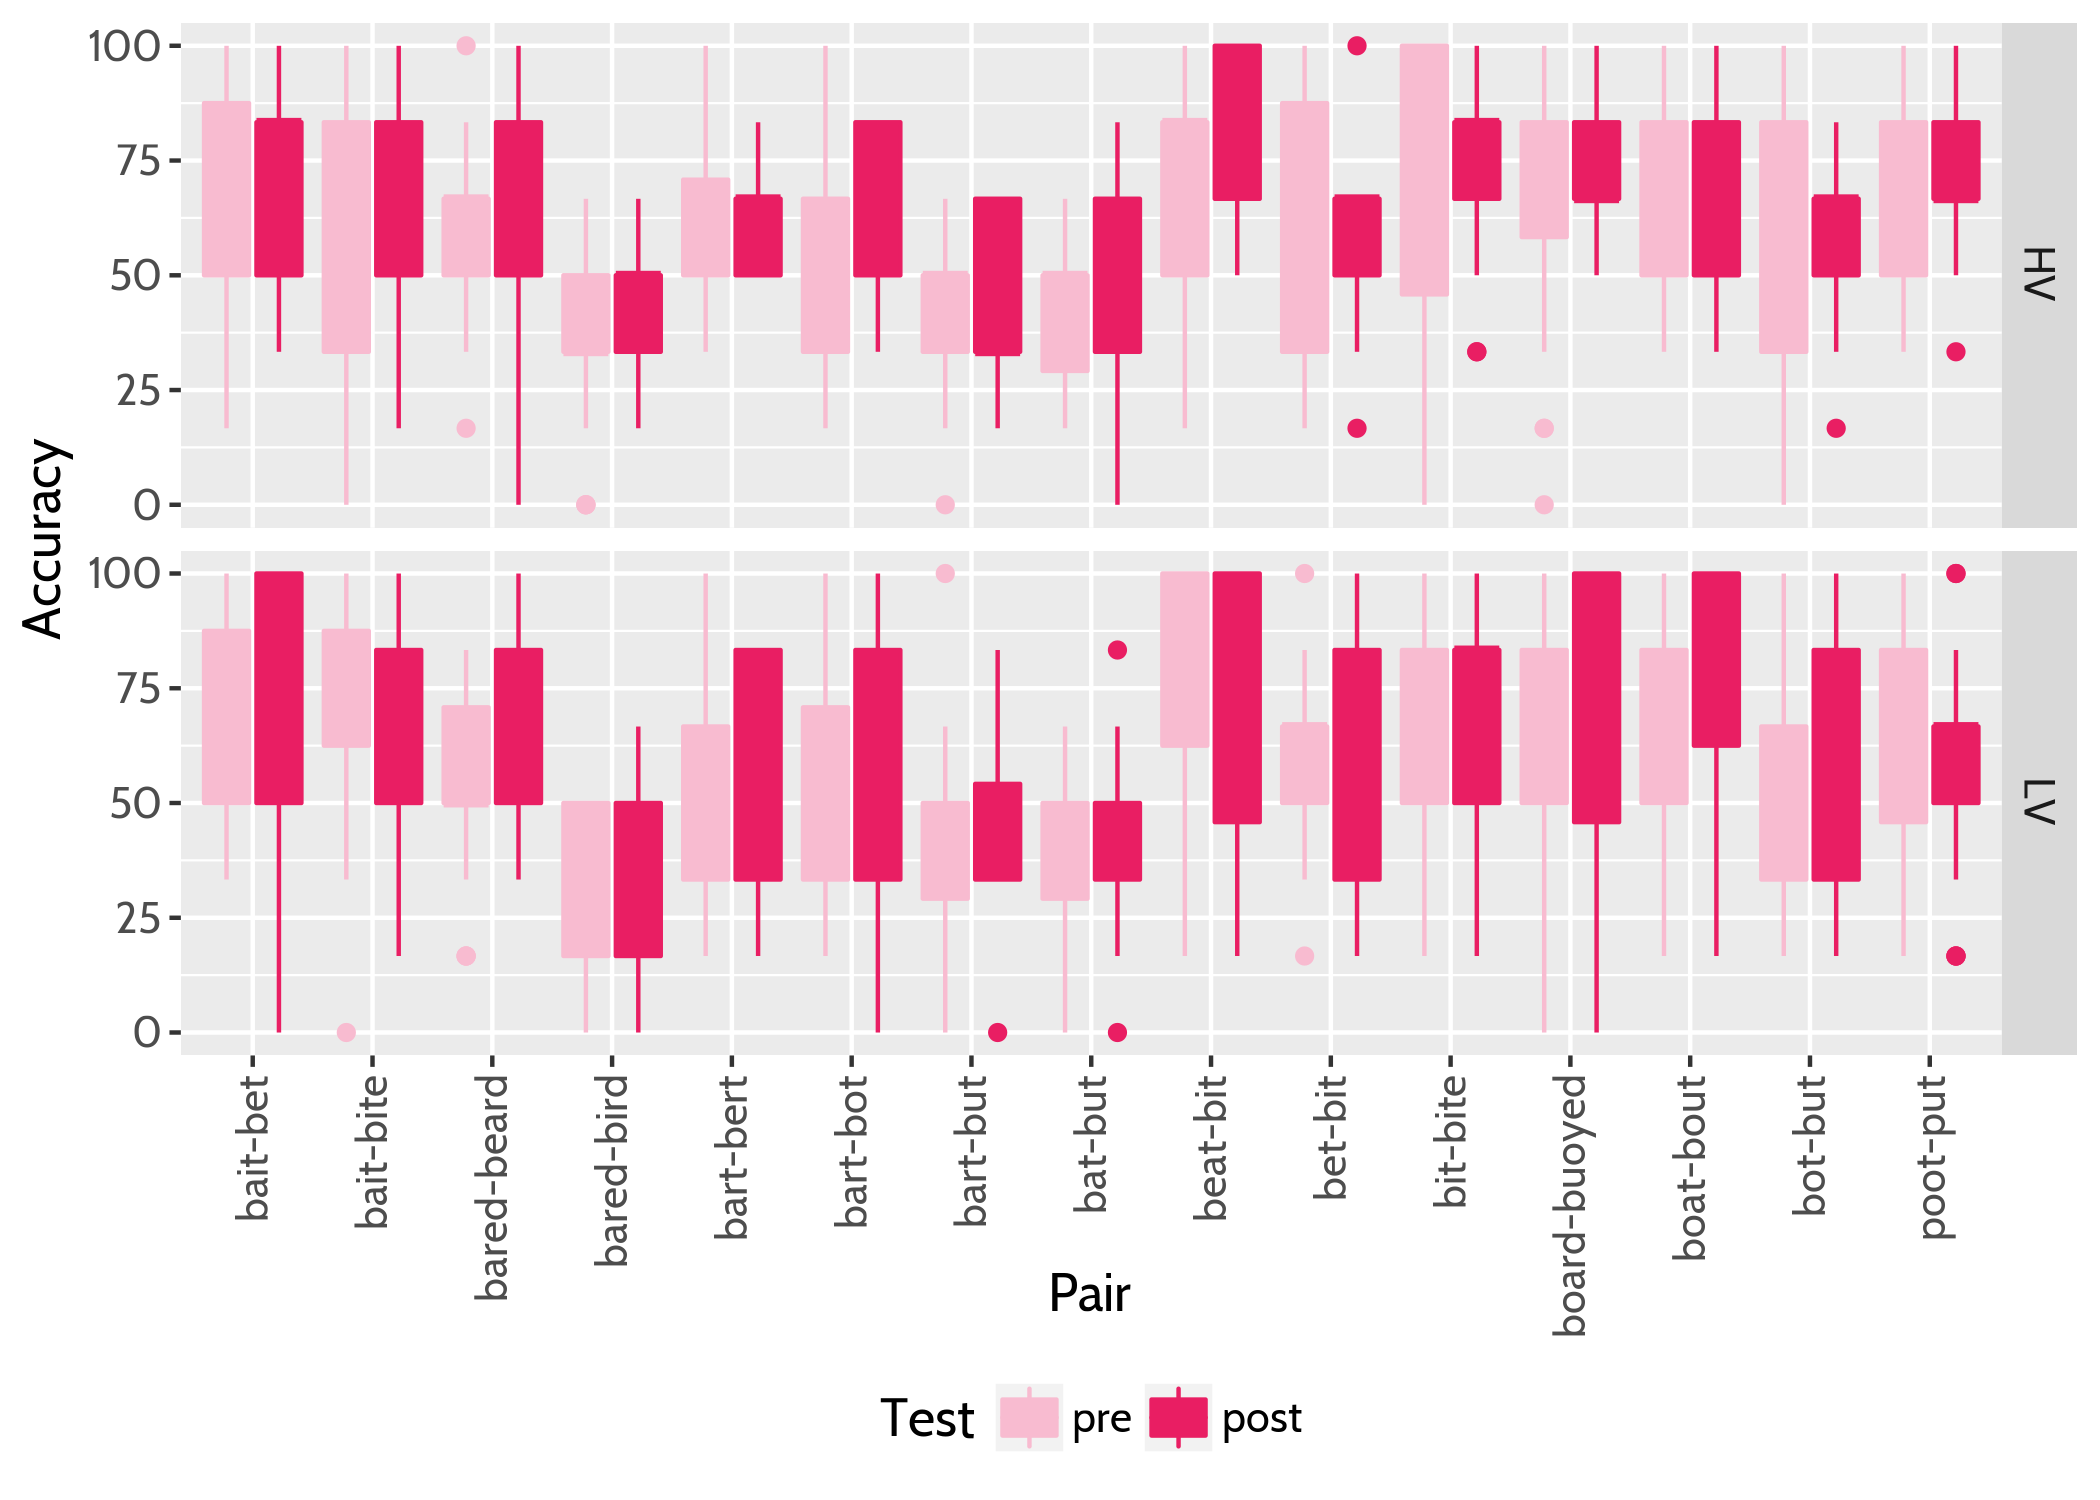
\includegraphics[width=\linewidth]{plots/axb-boxplot.png}
\caption{\label{axb-boxplot}
Box plots for the category discrimination task}
\end{figure}
\paragraph{Production (imitation task)}

\begin{figure}[h]
\includegraphics[width=\linewidth]{plots/vowel-plot.png}
\caption{\label{vowel-plot}
  Mean normalised formants for 11 monophthongs. SSBE formants
taken from \cite{hawkins_midgely_2005}}
\end{figure}


\begin{figure}[h]


\includegraphics[width=0.48\linewidth]{plots/ks-plot.png}
\hfill
\includegraphics[width=0.24\linewidth]{plots/duration-plot.png}
\includegraphics[width=0.24\linewidth]{plots/duration-model.png}
\caption{\label{ks-duration-plot}
  Distance between monophthongs produced by participants and SSBE speakers (left)
and monophthong duration for the participants (right)}
  \end{figure}

\begin{itemize}
\item Both LV and HV children show changes in most vowel production
between pre- and post- test (figure~\ref{vowel-plot})
\item
Kolmogorov-Smirnov (K-S) distance between children and SSBE
speaker's f1
decreases between pre- and post- test (figure~\ref{ks-duration-plot} left) although
this is not significant

\item
 Monophthong duration (figure~\ref{ks-duration-plot} right)
 increases significantly between pre- and post- test
 (F=68.532, p <0.0001)
\end{itemize}
  \end{block}





\begin{block}{Conclusions}

\end{block}

\begin{block}{References}
  \renewcommand\bibfont{\tiny}
  \printbibliography
\end{block}

\textbf{Acknowledgements}

  This work was supported by
  grant G-474-270-38 from King Abdulaziz University

\end{column}

\end{columns}

\end{frame}

\end{document}
